% ---------------------------------------------------
% ----- Main document of the template
% ----- for Bachelor-, Master thesis and class papers
% ---------------------------------------------------
%  Created by C. Müller-Birn on 2012-08-17, CC-BY-SA 3.0.
%  Last upadte: C. Müller-Birn 2015-11-27
%  Freie Universität Berlin, Institute of Computer Science, Human Centered Computing. 

\documentclass[pdftex,a4paper,12pt,DIV=calc,BCOR=5mm,twoside,smallheadings,titlepage]{scrbook}   
% ----- weitere Optionen 
%draft,			% Entwurfsmodus zum Anzeigen zu leerer/voller Boxen 
%DIV=calc
%DIV12,			% Seitengröße (siehe Koma Skript Dokumentation !) 
%BCOR5mm,		% Zusätzlicher Rand auf der Innenseite 
%twoside,		% Seitenränder werden an doppelseitig angepasst 
%fleqn,			% Formeln werden linksbündig (und nicht zentriert) angezeigt 
%titlepage,		% Titel wird in einer 'titlepage' Umgebung gesetzt 
%bigheadings,	% Große Überschriften (normal, small-headings) 
%halfparskip-	% Absatz wird nicht eingerückt, dafür aber um eine halbe Zeile nach unten gerückt
%
%---------------------------------------------------
%----- Packages
%---------------------------------------------------
%
\usepackage[T1]{fontenc} 
\usepackage[utf8]{inputenc}
\usepackage[english]{babel}  
\usepackage{ae}   
\usepackage{enumitem}
\usepackage{todonotes}
\usepackage{fancyhdr} % Define simple headings 
\usepackage{xcolor}
\usepackage{color}
\usepackage{url}
\usepackage{listings}
%\usepackage{vmargin} % Adjust margins in a simple way
%
\usepackage{amsmath}			% MUSS vor fontspec geladen werden
\usepackage{mathtools}			% modifiziert amsmath
\usepackage{amssymb}			% mathematische symbole, für \ceckmarks
\usepackage{amsthm}				% für proof
\usepackage{mathrsfs}	

\usepackage{graphicx}  
\usepackage{hyperref} 
\usepackage[noabbrev]{cleveref}
% turn all your internal references into hyperlinks
%\usepackage[pdfstartview=FitH,pdftitle={<<Titel der Arbeit>>}, pdfauthor={<<Autor>>}, pdfkeywords={<<Schlüsselwörter>>}, pdfsubject={<<Titel der Arbeit>>}, colorlinks=true, linkcolor=black, citecolor=black, urlcolor=black, hypertexnames=false, bookmarksnumbered=true, bookmarksopen=true, pdfborder = {0 0 0}]{hyperref}
%
\usepackage{tikz, ifthen}
%paragraph settings
%\setlength{\parskip}{1em}
% table settings 
\usepackage{booktabs}  
\usepackage{tabularx}  
\usepackage{rotating}
\usepackage{longtable}
%\usepackage{lscape}
\usepackage{multirow} %multi row
%\usepackage{rotating} %for rotating table
\usepackage{pdfpages}
\usepackage{float}
\usepackage{times}
\usepackage{cite}
\usepackage[section]{placeins}

%---------------------------------------------------
%----- PDF and document setup
%---------------------------------------------------
%
\hypersetup{
	pdftitle={Are We Explaining the Data or the Model? Concept-Based Methods and Their Fidelity in Presence of Spurious Features Under a Causal Lense},  % please, add the title of your thesis
    pdfauthor={Lilli Joppien},   % please, add your name
    pdfsubject={Master thesis, Institute of Computer Science, Freie Universität Berlin}, % please, select the type of this document
    pdfstartview={FitH},    % fits the width of the page to the window
    pdfnewwindow=true, 		% links in new window
    colorlinks=false,  		% false: boxed links; true: colored links
    linkcolor=red,          % color of internal links
    citecolor=green,        % color of links to bibliography
    filecolor=magenta,      % color of file links
    urlcolor=cyan           % color of external links
}
% 
%---------------------------------------------------
%----- Customize page size
%---------------------------------------------------
\usepackage[top=2cm,right=3cm,bottom=4cm,left=4cm]{geometry}    
%
%---------------------------------------------------
%----- Customize header and footer\pagestyle{fancy} 
%---------------------------------------------------
\pagestyle{fancy}

\fancyhf{}  % delete all existing header formating

\fancyhead[LE]{\leftmark}  % represent the current chapter heading in uppercase
\renewcommand{\chaptermark}[1]{ % adapt the shown chapter name: show it in lower case and with chapter number 
\markboth{\thechapter.\ #1}{}}   

\fancyhead[RO]{\rightmark}   % % represent the current section heading in uppercase 
\renewcommand{\sectionmark}[1]{% adapt the shown section name: show it in lower case and with section number 
\markboth{\thesection.\ #1}{}}

\renewcommand{\headrulewidth}{0pt} % remove lines from header
\renewcommand{\footrulewidth}{0pt} % remove lines from header

% independence sign _||_
\newcommand\independent{\protect\mathpalette{\protect\independenT}{\perp}}
\def\independenT#1#2{\mathrel{\rlap{$#1#2$}\mkern2mu{#1#2}}}

% have text above and below variable
\newcommand\stackequal[2]{%
  \mathrel{\stackunder[2pt]{\stackon[4pt]{=}{$\scriptscriptstyle#1$}}{%
  $\scriptscriptstyle#2$}}}
% declare my measures as variables to have text above and below them 
\DeclareMathOperator*{\MLC}{MLC}
\DeclareMathOperator*{\MAC}{MAC}
\DeclareMathOperator*{\RMA}{RMA}
\DeclareMathOperator*{\RRA}{RRA}
\DeclareMathOperator*{\PG}{PG}

\fancyfoot{} % delete all existing footer formating
\fancyfoot[LE,RO]{\thepage} % put page number on the left on even page and right on odd page
%
%---------------------------------------------------      
%----- Settings for word separation  
%---------------------------------------------------      
% Help for separation (from package babel, section 22)):
% In german package the following hints are additionally available:
% "- = an explicit hyphen sign, allowing hyphenation in the rest of the word
% "| = disable ligature at this position. (e.g., Schaf"|fell)
% "~ = for a compound word mark without a breakpoint (e.g., bergauf und "~ab)
% "= = for a compound word mark with a breakpoint, allowing hyphenation in the composing words
% "" = like "-, but producing no hyphen sign (e.g., und/""oder)
%
% Describe separation hints here:
\hyphenation{
% Pro-to-koll-in-stan-zen
% Ma-na-ge-ment  Netz-werk-ele-men-ten
% Netz-werk Netz-werk-re-ser-vie-rung
% Netz-werk-adap-ter Fein-ju-stier-ung
% Da-ten-strom-spe-zi-fi-ka-tion Pa-ket-rumpf
% Kon-troll-in-stanz
}
%
%---------------------------------------------------
%----- Restricting including files   
%---------------------------------------------------
% Only files listed here will be included in the PDF document!
% In order to only partially translate the document, for example for bug-fixing, 
% it might be useful to comment out some of the documents.
\includeonly{
title,
declaration,
abstract_en,
abstract_de,
introduction,
background,
problem_setting,
method,
results,
conclusion,
appendix
}

%%%%%%%%%%%%%%%%%%%%%%%%%%%%%%%%%%%%%%%%%%%%%%%%%%%%%%
% The content part of the document starts here! %%
%%%%%%%%%%%%%%%%%%%%%%%%%%%%%%%%%%%%%%%%%%%%%%%%%%%%%%

\begin{document}
%---------------------------------------------------
%----- Listing and color definition   
%---------------------------------------------------
\definecolor{red}{rgb}{.8,.1,.2}
\definecolor{blue}{rgb}{.2,.3,.7}
\definecolor{lightyellow}{rgb}{1.,1.,.97}
\definecolor{gray}{rgb}{.7,.7,.7}
\definecolor{darkgreen}{rgb}{0,.5,.1}
\definecolor{darkyellow}{rgb}{1.,.7,.3}
\lstloadlanguages{C++,[Objective]C,Python}

\definecolor{codegreen}{rgb}{0,0.6,0}
\definecolor{codegray}{rgb}{0.5,0.5,0.5}
\definecolor{codepurple}{rgb}{0.58,0,0.82}
\definecolor{backcolour}{rgb}{0.95,0.95,0.92}

\lstdefinestyle{mystyle}{
    backgroundcolor=\color{backcolour},   
    commentstyle=\color{codegreen},
    keywordstyle=\color{magenta},
    numberstyle=\tiny\color{codepurple},
    stringstyle=\color{codepurple},
    basicstyle=\ttfamily\footnotesize,
    breakatwhitespace=false,         
    breaklines=true,                 
    captionpos=b,                    
    keepspaces=true,                 
    %numbers=left,                    
    %numbersep=5pt,                  
    showspaces=false,                
    showstringspaces=false,
    showtabs=false,                  
    tabsize=2
}
% TIKZ STUFF
\usetikzlibrary{arrows.meta,arrows}
\usetikzlibrary{shapes}

\lstset{style=mystyle}
%---------------------------------------------------
%----- Title and declaration   
%---------------------------------------------------
\pagenumbering{alph}
% ---------------------------------------------------
% ----- Title page of the template
% ----- for Bachelor-, Master thesis and class papers
% ---------------------------------------------------
%  Created by C. Müller-Birn on 2012-08-17, CC-BY-SA 3.0.
%  Freie Universität Berlin, Institute of Computer Science, Human Centered Computing. 
%

\title{
{\small Masterarbeit}\\
{\small Climate Informatics TU Berlin / Causal Inference Group DLR Jena}\\
[7ex]
{Are We Explaining \\ the Data or the Model?} \\
[1ex]
{\LARGE Concept-Based Methods and
Their Fidelity in Presence of Spurious Features Under a Causal Lense.}}

\author{
{\emph{\normalsize Lilli Joppien}}\\
[18ex]   
{\normalsize Betreuer*innen: Oana-Iuliana Popescu, Simon Bing} \\
{\normalsize Erstgutachter: Prof. Dr. Jakob Runge} \\
{\normalsize Zweitgutachter: Prof. Dr. Tim Landgraf (oder Georges Montavon?) }}
\vspace{6ex}
\date{\normalsize Berlin, \today}
\maketitle



%---------------------------------------------------
%----- Change word wrapping if it is too annoying 
%---------------------------------------------------
%\emergencystretch 3em
%\raggedright
%\sloppy
\hyphenpenalty=4000
\tolerance=1000

%---------------------------------------------------
%----- Abstracts in English and German   
%---------------------------------------------------

\subsection*{Abstract}
\begin{itemize}
    \color{red}
    \item The abstract must not contain references, as it may be used without the main article. It is acceptable, although not common, to identify work by author, abbreviation or RFC number. (For example, "Our algorithm is based upon the work by Smith and Wesson.")
    \item Avoid use of "in this paper" in the abstract. What other paper would you be talking about here?
    \item Avoid general motivation in the abstract. You do not have to justify the importance of the Internet or explain what QoS is.
    \item Highlight not just the problem, but also the principal results. Many people read abstracts and then decide whether to bother with the rest of the paper.
    \item Since the abstract will be used by search engines, be sure that terms that identify your work are found there. In particular, the name of any protocol or system developed and the general area ("quality of service", "protocol verification", "service creation environment") should be contained in the abstract.
    \item Avoid equations and math. Exceptions: Your paper proposes E = m c 2.
\end{itemize}

\subsubsection*{Motivation}
\begin{itemize}
    \item explainable AI shows great progress in visualizing how neural networks see/decide
    \item however there have been many criticisms and some argue that the XAI methods don't show what is actually seen by the NN and rely more on hyperparameters or the data itself.
    \item For example, it is known that some attribution methods do not react well to constant vector shifts in the data which do not affect prediction.
    \item it is especially unclear how the explanation method deals with causal constructs: is there a difference between how it displays cause and effect, can it find important interactions between 2 variables or find spurious correlations?
    \item we want to identify how the ground truth biasedness of a dataset interacts with the biasedness of the model and the biasedness of the explanation
    \item for general attribution methods it has been shown that heatmaps can be misleading. If the spurious feature has any correlation with the core feature, it will often have importance assigned. In many instances, the spurious feature comes as a watermark which is easy to identify for humans and usually spatial compact. Consequently its importance can be overestimated when looking at a general heatmap of an image.
    \item Looking at individual concepts with their relevances and specific heatmaps has the potential to identify which of the features (core or spurious) is actually most relevant.
\end{itemize}

\subsubsection*{Problem Statement}
\begin{itemize}
    \item investigate the example of CRP, a recent method which takes the popular Layer-Wise Relevance Propagation to the next level, by producing conditional attributions for neurons or sets of neurons coined "concepts"
    \item find out, whether the heatmaps or relevances produced by this algorithm have a connection either to the causal ground truth of data or the "causal pathways" in the NN
    \item quantify the relationship between the causal model, the learned representation and the CRP explanation.
\end{itemize}

\subsubsection*{Approach}
\begin{itemize}
    \item for validation purposes very simple disentangling dataset DSPRITES
    \item introduce "causal" biases into dataset, by adding small watermark not uniformly to certain images
    \item use a very small neural network, which is strong enough to perform well at the task but learns the spurious feature once it becomes overwhelmingly correlated to the core feature.
    \item intervene on the bias strength to see how 
    \item \textit{do causality lol}
\end{itemize}

\subsubsection*{Results}
\begin{itemize}
    \item does CRP succeed in identifying the true biasedness of the model
    \item what do we want to explain
    \item does this result generalize for other attribution methods, data, SCMs?
\end{itemize}

\subsubsection*{Conclusions}
\begin{itemize}
    \item found a new benchmark measure to combat the critique about the robustness and fidelity of especially concept-based methods.
    \item from that new method a way to enrich or improve those methods arises
    \item it is important to look at explanations in a more causal light because that is what they are ought do be doing
    \item what else needs to be done especially
\end{itemize}

% ---------------------------------------------------
% ----- Abstract (German) of the template
% ----- for Bachelor-, Master thesis and class papers
% ---------------------------------------------------
%  Created by C. Müller-Birn on 2012-08-17, CC-BY-SA 3.0.
%  Freie Universität Berlin, Institute of Computer Science, Human Centered Computing. 
%
\pagestyle{empty}

\subsection*{Zusammenfassung}
Methoden der erklärbaren künstlichen Intelligenz (Explainable Artificial Intelligence, XAI), insbesondere lokale Wichtigkeitszuordnung, sind ein beliebtes Instrument zur Visualisierung der Bedeutung von Eingangsmerkmalen wie Pixeln für ein neuronales Netz.
Folglich gibt es eine wachsende Zahl von Arbeiten, die diese Wichtigkeitszuordnung und ihre Visualisierung sowie im speziellen konzeptbasierte Methoden rigoroser evaluieren und ihre Grenzen und Nachteile aufzeigen. In diesem Bereich hat die Anwendung des Kausalitätsrahmens basierend auf Pearls Arbeit an Zugkraft gewonnen, da Erklärungen ein inhärent kausales Konstrukt sind. Die kausale Auswertung von XAI wird häufig von künstlich generierten Benchmark-Datensätzen mit bekannten Generierungsvariablen begleitet, um die tatsächliche Funktionsweise eines neuronalen Netzes ermitteln zu können. 
Die neuere Erklärungsmethode Konzeptbedingte Relevanzpropagation (Concept Relevance Propagation, CRP) scheint den Menschen besser als reine Saliency-Visualisierungen in die Lage zu versetzen, zu erkennen, ob ein Modell verzerrt ist, basierend auf einer kleinen Nutzerstudie und qualitativen Untersuchungen. Bisher wurde dieses Potenzial aber nicht quantitativ evaluiert, vermutlich weil die relative Bedeutung von unerwünschten Merkmalen schwerer formal zu testen ist als die grundsätzliche Kohärenz zu einem trainierten Modell. 
Mit Hilfe eines kausalen Benchmark-Datensatzes untersuchen wir daher die Reaktion von Concept Relevance Propagation (CRP) auf eine Intervention in einem kausalen Modell. 
Unser kausaler Prozess führt eine Scheinkorrelation ein, mit einem Merkmal das keine direkte Beziehung zum wirklich wichtigen Merkmal hat, sondern durch einen Störfaktor mit ihm gekoppelt ist. Indem wir die Stärke dieser Kopplung kontinuierlich erhöhen, können wir analysieren, ob die Reaktion der Erklärung auf ein solches falsch korreliertes Merkmal der tatsächlichen Reaktion des Modells folgt. Zu diesem Zweck konstruieren wir eine Reihe von Metriken, die den Einfluss einer solchen Verzerrung sowohl auf die Erklärung als auch auf das Modell quantifizieren. Wir stellen fest, dass der gemessene kausale Effekt auf die Entscheidung des Modells und die Erklärung zum großen Teil übereinstimmen. Je abstrakter und menschlich interpretierbarer wir jedoch die Erklärung messen, desto weniger genau folgt sie der echten Wichtigkeit. Dieses Ergebnis ist besorgniserregend, da neuere Studien an Probanden gezeigt haben, dass die Salienz m

  
                                          
%---------------------------------------------------
%----- Directories   
%---------------------------------------------------

\frontmatter 
\pagenumbering{roman}

\tableofcontents
\setcounter{tocdepth}{2}   % reduce the included sections in the table of content

\listoffigures
\listoftables

%---------------------------------------------------
%----- Main part
%---------------------------------------------------
\mainmatter
\pagenumbering{arabic} 
\pagestyle{fancy} 

%\include{preface} 

\chapter{Introduction}\label{chapter:introduction}

\begin{itemize}
\color{red} 
    \item (1-2 pages)
    \item Context: make sure to link where your work fits in Problem: gap in knowledge, too expensive, too slow, a deficiency, superseded technology. Strategy: the way you will address the problem
    \item Outline of the rest of the paper: "The remainder of the paper is organized as follows. In Section 2, we introduce ..Section 3 describes ... Finally, we describe future work in Section 5." (Note that Section is capitalized. Also, vary your expression between "section" being the subject of the sentence, as in "Section 2 discusses ..." and "In Section, we discuss ...".)
    \item Avoid stock and cliche phrases such as "recent advances in XYZ" or anything alluding to the growth of the Internet. 
    \item Be sure that the introduction lets the reader know what this paper is about, not just how important your general area of research is. Readers won't stick with you for three pages to find out what you are talking about.
    \item The introduction must motivate your work by pinpointing the problem you are addressing and then give an overview of your approach and/or contributions (and perhaps even a general description of your results). In this way, the intro sets up my expectations for the rest of your paper -- it provides the context, and a preview.
    \item Repeating the abstract in the introduction is a waste of space.
\end{itemize}

AGAIN: structure what i need to say:
\begin{itemize}
    \item XAI is becoming bigger, so is its evaluation
    \item therefore recently more criticisms, especially about local attribution methods
    \item lack of proper evaluation, "circular criteria (such as fidelity and faithfulness Gevaert et al. (2022))", \cite{Adebayo2018, Sixt2020, Wilming2023} etc.
    \item crp attempts to alleviate some of that, going away from "where" question, which does not seem to hold much information in some cases, to "what" question (is this actually related to recent evaluation stuff???)
    \item therefore we want to evaluate whether crp actually manages to better identify biases using numerical measure
    \item for that we use a new approach with a causally generated ground truth of a simple dataset, otherwise numerical measure of "biasedness" would not be possible
    \item try to make this scm and images as close to a realistic image dataset as possible
    \item we don't attempt to measure importance of feature which is supposed to be important (core feature) but of clever-hans feature
    \item instead of having an either biased or unbiased dataset, we use coupling ratio
    \item it makes it theoretically possible to establish a sort of threshold for feature importance? e.g. if feature more important than core feature, or a third or something?
    \item REFER MORE TO \textit{Are We Explaining The Data Or The Model?}
    \item most other work either has known bias or not. but it is not necessarily quantified how much of that bias was learned by model. 
\end{itemize}

\section{Motivation and Context}
With the explosion in popularity of deep neural networks the need to explain those opaque, black-box models has risen too. Recently, explainable AI (XAI) methods have been scrutinized more closely. Although there is still no consensus on what exactly makes a \textit{good explanation}, numerous potential metrics for the faithfulness, robustness and interpretability of explanations have been made \cite{?}. A promising branch of research seems to be the evaluation of explainable AI methods with causal methods. After all, explanations are, or at least should be, intrinsically causal constructs \cite{Woodward2004, Halpern2005, Schoelkopf2019}.\\

Due to the stronger focus on evaluation of XAI, amongst other methods also local attribution methods have come under criticism for their general lack of faithfulness to the model they are trying to explain \cite{Adebayo2018, Karimi2023}. Also, some methods class-insensitivity \cite{Sixt2020} and their failure in presence of suppressor variables \cite{Wilming2023} and in the \textit{limit of simplicity} \cite{Kindermans2017} have been examined.  Other authors have criticized the lack of comparative user-guided evaluation of explanation methods \cite{Rong2023}. \\

As local attribution methods, especially back-propagation methods, create visually compelling results through attribution maps, they have still become a staple for many AI practitioners, especially for computer vision tasks. 

The recent \textit{glocal} attribution method \textit{Concept-Relevance-Propagation (CRP)} introduced in \cite{Achtibat2022} has been developed for a more fine-grained explanation of a neural networks decisions. Instead of producing one attribution map explaining the overall prediction output such as LRP \cite{Bach2015}, each \textit{concept} in some hidden layer of the network gets assigned a conditional relevance and its own saliency map. In addition to the saliency maps, the relevance scores also act as a metric to maximize when searching representative samples for each of the concepts. According to the authors, through this more detailed explanation one can not only understand \textit{where} a model sees the most relevant features, but also \textit{what} features are relevant in this area. Their pre-assumption is, that the deeper layers of models represent concepts which are human-understandable and therefore aid in the explanation of what the model predicts. In qualitative examinations, as well as a human evaluation study \cite{Achtibat2023}, they find that \textit{Clever-Hans} (i.e. spuriously correlated) features are easier to identify with the concept-based approach and their relevance better determined in comparison to other local attribution methods. Finding whether a background or spuriously correlated feature is biasing a model is in our opinion one of the most important applications of XAI.
\\

Here, we therefore make the attempt to evaluate yet another desirable characteristic of XAI: that its sensitivity to spurious feature importance closely follows that of the network it is trying to explain. The general sensitivity or faithfulness to a model has been studied with varying methods, most often creating perturbations in the input or model at the \textit{important} feature and testing the decline in accuracy. Some recent works have also evaluated an explanations feature importance when spuriously correlated features are present \cite{Yang2019,Kim2018,Parafita2019,Reimers2020,Singla2022}. Arguably, explanations having high fidelity is especially crucial when identifying and quantifying spurious correlations a model has learned. Confirming that the true feature has some importance is not as convincing of an explanation if the importance of other features is not compared to it.
We believe that to establish the true effect of a spuriously correlated feature on a models prediction, it is interesting to also look at it in a continuous and relative fashion. 
In a realistic setting it is hard for a model to not have learned at least some bias. This is especially true because it seems impossible even for humans to know the \textit{true causal model} of how e.g. images are created. So in accordance with ideas of \textit{fairness} it seems impossible to aim for completely unbiased models, as they would need to have all knowable and unknowable knowledge of the universe to not predict 'out-of-distribution'. Instead, one needs to define a measurable threshold of biasedness, which is acceptable for a specific task.  

Therefore we will extend previous work on evaluating the explanation methods fidelity in the presence of Clever-Hans features, by using a known causal model. We extend a simple benchmark dataset with known ground truth to have a structural causal model which generates the data.
While the \textit{core} feature actually determines the class other, \textit{spurious} features are still present and correlate with the core feature in aknown way \cite{Singla2022}.
Knowing the generating factors helps to quantify the ground-truth feature importance of not only the core and the spurious feature but also irrelevant features as a baseline.


With the aim of evaluating fidelity in the presence of a spuriously correlated feature, a zoo of models is trained with varying coupling ratios. Ground-truth biasedness is calculated for each model and each feature. In expectation, the models importance for the core feature declines and for the spurious feature increases as the coupling ratio rises. 


If CRP indeed produces an accurate explanation, more concepts should assign higher relevance to the bias feature the stronger the bias impacts the prediction of the model. It is important to note, that the model might accurately predict based on the real feature even though the bias is strong, when there are enough counterexamples. \Cref{fig:tesfigure} shows the non-linear interaction between prediction accuracy and coupling ratio.
Now the question is, whether CRP can correctly identify this non-linear relationship or whether CRPs attribution to the spurious feature will more closely follow its actual presence in the data. 
In other words: Does CRP learn the causal effect of the spurious feature on the model or just the causal effect within the data? Our goal is to quantify the effect that CRP actually has on human understanding. So even if the overall importance of the watermark can be either denied or affirmed, the numeric importance might not be the same as what a user can see and find through heatmaps, relevance hierarchies and relevance maximization image sets. Therefore it is necessary to develop methods which quantify human understanding of biasedness?  

\section{Contributions}
\todo{refine strategy based on what i actually did}
\begin{itemize}
    \item Construct a causal model of the explanation generation process
    \item Construct a causal data generating model embedded into the larger model
    \item Train a succession of neural network instances by intervening on a meta variable that determines the correlations in the data distribution
    \item Establish a ground-truth of model accuracy and feature importance in relationship to the intervened factor
    \item Evaluate explanations in a concept-based approach using concept relevance propagation (CRP)
    \item Construct X metrics describing the effect of the intervention on the explanations feature importance 
    \item Compare the effect of the intervention on model importance and explanation importance
\end{itemize}

\section{Outline}
To further motivate this approach we will in the following summarize previous work on XAI, evaluation of XAI, causality and their combination \cref{chapter:background}. We will also lay down the theoretical framework of the XAI method and the causal concepts studied here. \Cref{chapter:method} introduces the causal explanation generation process, and how the benchmark dataset embeds into it. It also describes the methods used to establish a ground-truth \textit{feature importance} as well as metrics for measuring feature importance in our explanation. The architecture and training of the DNN model and other details of the conducted experiment are detailed here too. Finally the different measures are compared and visualized in \cref{chapter:results} and discussed in \cref{chapter:conclusion}.

\chapter{Preliminaries}\label{chapter:background}

To embed this thesis into existing work, we will first give a short introduction to the field of neural networks and XAI. This will be followed by a more in-depth look at layer-wise and concept relevance propagation which is to be evaluated in our analysis. We will then introduce the main ideas of the causality framework we are going to use and how it has been previously applied in the context of (the evaluation of) XAI. 


\section{Neural Networks}
Among the many machine learning approaches that have been developed, the most popular, but arguably most opaque, are deep neural networks. In general, a neural network consists of neurons, which are computational nodes organized in layers. In the most simple forward pass, each neuron weighs its inputs, offsets them with a bias and then feeds the result through a non-linear function. This is repeated in the next layer of neurons until the output layer is reached. During training, a loss function between the predictions for data instances and their true labels is optimized by back-propagating its gradient and updating the internal weights and biases. For specifics on successful architectures and training procedures we refer to text books on deep learning, for example by \cite{Goodfellow2016}. When trained with enough data, the weights and biases together approximate a high-dimensional and non-linear function describing the training data. This function however is hard to analyze and interpret for humans when trying to understand the reasoning of the network. This lead to the emergence of many explanation methods attempting to uncover those inner workings in a human-interpretable way.


\section{Explainable Artificial Intelligence}
With the field of machine learning and particularly complex deep neural network models continuously expanding, so is the demand for explanations of these models.
As especially neural networks are so called \textit{black boxes} that inhibit a human understanding of their results, plenty of explanation methods have been developed, summarized under the term XAI. The sub-field of interpretable AI aims to create inherently transparent models, but they may come with a decrease in performance \cite{Lipton2018}. Therefore, many XAI methods are explaining what a model has learned \textit{post-hoc}, either model-agnostic by only evaluating decisions based on input data or model-specific by using information on latent parameters of a model.


The methods can also be generally divided into local and global approaches. Local methods aim to explain the decision making for one specific example, like one image in a computer vision task, typically by attributing importance to input features like pixels. Global methods on the other hand make more general interpretations of a model, for example, which abstract features are identified in the decision-making process. An example is activation-maximization \cite{Nguyen2016} which finds prototypical instances of classes or latent filters by maximizing their activation. 

The first (local) category prominently includes saliency map methods, which are most often applied on computer-vision tasks, where they assign importance to pixels or regions of a sample image, creating a heatmap. 
The importance is computed through forms of back-propagation \cite{Bach2015,Zhang2016,Kindermans2017}, with the help of gradients \cite{Sundararajan2017,Smilkov2017} or in a model-agnostic way by perturbing or occluding parts of the input \cite{Lundberg2017,Zeiler2013,Zintgraf2017,Agarwal2020}. Resulting saliency maps may generate insight into the locality of important objects. However, this is usually only one facet of understanding the decision-making of a model, especially for people not familiar with the data domain. If the location of importance is identified, it is still not clear \textit{what} is important in this region.   

Recently, there has therefore been a surge in combining local and global methods, through embedding local attribution maps into more global strategies of a model. \cite{Achtibat2022} use local attribution methods to aid in finding human-interpretable, abstract concepts that a model encodes. As a \textit{concept-based} method it utilizes the latent space of a neural network to find abstract components in the input space encoded by the model \citep{Bau2017,Bau2020,Kim2018, Ghorbani2019, Zhang2021, Fel2023a}. 
Some approaches are partly supervised, in that a human has to first define what a concept is, e.g. by labelling a ground truth or by selecting a few images that belong to a certain concept \citep{Kim2018, Singla2022}. Others try to make sense of either the latent space spanned by the \textit{concept activation vectors} or the space of per-pixel attributions, for example, by clustering it \citep{Lapuschkin2019,Vielhaben2023} and disentangling and visualizing concepts  \citep{Ghorbani2019,Zhang2021,Leemann2023,Fel2023,Chormai2022, Singla2022}.

\subsection{Layer-wise Relevance Propagation}\label{section:lrp}
Layer-wise Relevance Propagation (LRP) \citep{Bach2015} is the basis for Concept Relevance Propagation (CRP), which we will analyze in this thesis, and is among the most highly cited local attribution methods in XAI. Having been introduced almost 10 years ago, it has been justified mathematically with Deep Taylor Decomposition \citep{Montavon2017}. It belongs to the class of (modified) back-propagation methods which propagate a custom value back to the input through a set of backpropagation rules. A visual representation of this strategy can be found in \cref{fig:crp_vs_lrp} \textbf{(a)}. Like other saliency methods, LRP is commonly used in computer vision tasks to attribute importance to each pixel in an image, which can then be visualized as a heatmap, but is also applicable to other data formats. In the following we will summarize the basic functioning of LRP for neural networks as described by \cite{Bach2015}:

The general idea is to find how input features contribute to a prediction in relation to a root point of maximal uncertainty $f(\mathbf{x}_0) = 0$ so that the positive or negative relevances of separate pixels roughly sum up to the output for that instance:
\begin{equation}\displaystyle
    f(\mathbf{x}) \approx \sum_{d \in \mathbf{x}} R_d
\end{equation}

LRP assumes that the model has multiple layers of computation it can be decomposed into, starting from the input layer, for example the pixels of an image, to all latent layers $\ell$ and finally to the output layer. Further, each of those layers has $|\ell|$ dimensions for which a relevance score $R^{\ell}_d$ can be determined so that the following equation holds:
\begin{equation}
    f(\mathbf{x}) = ... = \sum_{d \in \ell+1} R^{(\ell+1)}_d =  \sum_{d \in \ell} R^{(\ell)}_d = ... =  \sum_{d} R^{(1)}_d
\end{equation}

In neural networks, the general forward step for a layer $j$ means weighing the previous layer's $i$ outputs $f_i(\mathbf{x})$ with the current layer's weights $z_{ij} = f_i(\mathbf{x}) w_{ij}$, summing the results for all connected neurons and their bias $z_{j} = \sum_{i} z_{ij} + b_j$ and running this through a non-linear activation function $f_j(\mathbf{x}) = \sigma (z_j)$.
The intuition then is to follow the flow of relevance from the output, where usually the prediction value $f(\mathbf{x})$ is taken to initialize the relevance $R^(1)_d$, back to the input layer by decomposition. In the simplest case relevance is proportionally propagated back to the previous layer where the relevance of all connected neurons is aggregated in the following way:
\begin{equation}\label{eq:basic_attribution_rule}
    R_i = \sum_{j}  R_{i \leftarrow j} = \sum_{j} \frac{z_{ij}}{z_j} R_j
\end{equation}

To apply LRP, certain best practices and rules have been established \citep{Kohlbrenner2020, Montavon2019, Samek2021}. Depending on the type and location of a layer within a neural network the propagation rule can be varied. In this thesis we stick to the method that the authors of CRP use, namely the composite $LRP_{\epsilon-z+-\flat}$-rule (read ``epsilon-plus-flat''), which is recommended by \cite{Kohlbrenner2020} and composes different rules for different parts of the model, further described in the \cref{appendix:lrprules}.

\subsection{Concept Relevance Propagation}\label{section:crp_background}
Concept Relevance Propagation, a recent contribution by \cite{Achtibat2022}, is called a \textit{glocal} XAI method by its authors, extending on the established local attribution technique Layerwise Relevance Propagation (LRP) \cite{Bach2015} and applying other more global methods like \textit{relevance maximization}. 
Layerwise Relevance Propagation, as a local XAI method, produces saliency maps for single data samples through a modified backpropagation process further described in the previous \cref{section:lrp}. By filtering on subsets of latent features within the layers of the model during this modified backpropagation, CRP yields saliency maps which could, in principle, produce more targeted explanations. With the help of global feature visualization methods CRP's authors try to go beyond the pure ``where'' of saliency maps, towards a ``what'', explaining which (human understandable?) concepts a model has recognized in a specific image region. This idea is integrating into the mentioned growing field of \textit{concept-based} explanation methods.

\begin{figure}[t!]
    \centering
    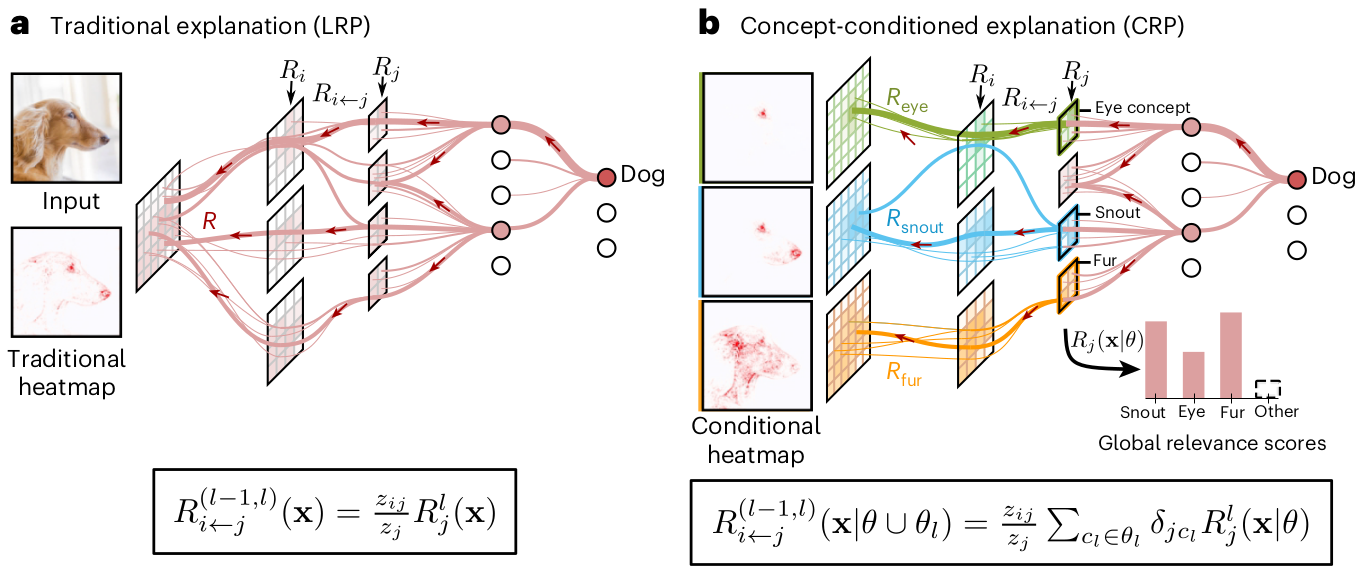
\includegraphics[width=0.9\textwidth]{thesis_latex_template/pics/crp_vs_lrp_from_paper.png}
    \caption[CRP vs. LRP]{\textbf{a} (LRP): output value back-propagated through network, \textbf{b} (CRP): output conditioned on concepts, i.e., certain neurons are masked out in back-propagation (taken from \cite{Achtibat2023}'s more recent paper summarizing Concept-Relevance Propagation)}
    \label{fig:crp_vs_lrp}
\end{figure}

LRP aggregates the significance of all latent layers and their neurons into one importance map, where the intermediate layers' outputs are merely a side-product of the computation.
\cite{Achtibat2022} propose in their work to use those intermediate results to disentangle the attributions. In LRP the initialization at the output layer usually takes the value of one class output $y= f(\mathbf{x})$ w.r.t input $\mathbf{x}$, all other output neurons set to zero, and thereby produces a class-conditional attribution ($R(\mathbf{x}|y)$). A similar thing can be done in latent layers too. Although it is yet unclear how to interpret the attribution to these hidden features, the authors of CRP propose to obtain importance scores for them by computing \textit{(multi-)concept-conditional} relevances $R(\mathbf{x}|\theta)$. The variable $\theta$ here describes a set of conditions $c_{\ell}$ which in essence filters for certain ``concepts'' (neurons) in potentially multiple layers by masking out all other neurons' contributions:

\begin{equation}\displaystyle
    R^{(\ell-1, \ell)}_{i \leftarrow j} (\mathbf{x} | \theta \cup \theta_{\ell}) = \frac{z_{ij}}{z_j} \cdot \sum_{c_{\ell} \in \theta_{\ell}} \delta_{jc_{\ell}} \cdot R^{\ell}_j (\mathbf{x} | \theta )
\end{equation}

Here, $\delta_{jc_l}$ is the Kronecker-Delta selecting the relevance $R^l_j$ of feature $j$ in layer $l$ if that index is in the condition $c_l$, masking out all other features in that layer. If no condition is set for a particular layer, the relevance from that layer is not masked. The authors note that conditions compare to logical OR operations within the same layer and to AND operations across layers. 

\subsubsection{Interpretation Techniques with CRP}
Heatmaps produced by conditional attribution can be looked at in a similar fashion to the traditional class-specific heatmaps produced by LRP. The hindrance is that the meanings of the latent features, that are conditioned on, are not known so it is unclear how to interpret the importance of some pixels for concept $c$ in layer $\ell$. For large, complex models some human-understandable concepts can emerge in hidden layers from simpler, more local, concepts in earlier to more abstract concepts in later layers \citep{Bau2017, Hohman2020, Olah2017, Bau2020}. However, this is not a reliable fact and seems to regularly fail, especially for smaller models or simpler problems, as is becoming visible in some of the examples in this work and other evaluations \citep{Kim2018,Singla2022, Sixt2022a}.

CRP's authors therefore construct a framework for the understanding of these latent features. The global method of \textit{Activation Maximization} \citep{Nguyen2016} is used to find the samples for which the neuron (-set) of a concept has the highest activation. They extend on the idea of it when proposing \textit{Relevance Maximization}, where samples maximize the conditional relevance of a concept $c$ instead of the activation for that filter. Both methods yield a set of samples (see \cref{fig:act_rel_max}), which can be enhanced further by masking out the less relevant parts of the image. This way, class- and concept-specific reference samples are collected. They also recommend carefully selecting or extending the pool of samples to maximize on so as to improve the diversity of references. By maximizing the \textit{relevance} of a filter instead of its activation for a specific class, the authors claim to find a more outcome-specific illustration. The success of this technique depends on whether humans are able to identify the concept strongest overlapping within the reference set though. It can be seen that this is not a trivial task in the given sample (\cref{fig:act_rel_max}) and we will extend on this within our experiments later. 

\begin{figure}[t!]
\centering
\begin{minipage}{0.48\textwidth}
    ActMax 700k images \\
	\includegraphics[width=\textwidth]{thesis_latex_template/pics/act_max_no_diversity_uncropped.png}\\
    ActMax 300 images \\
	\includegraphics[width=\textwidth]{thesis_latex_template/pics/act_max_with_diversity_uncropped.png}\\
    RelMax 700k images\\
	\includegraphics[width=\textwidth]{thesis_latex_template/pics/rel_max_no_diversity_uncropped.png}\\
    RelMax 300 images \\
	\includegraphics[width=\textwidth]{thesis_latex_template/pics/rel_max_with_diversity_uncropped.png}
\end{minipage}
\begin{minipage}{0.48\textwidth}
    zoomed into receptive field \\
	\includegraphics[width=\textwidth]{thesis_latex_template/pics/act_max_no_diversity.png}\\
    zoomed into receptive field \\
	\includegraphics[width=\textwidth]{thesis_latex_template/pics/act_max_with_diversity.png}\\
    zoomed into receptive field \\
	\includegraphics[width=\textwidth]{thesis_latex_template/pics/rel_max_no_diversity.png}\\
    zoomed into receptive field \\
	\includegraphics[width=\textwidth]{thesis_latex_template/pics/rel_max_with_diversity.png}
\end{minipage}
\caption[ActMax vs. RelMax]{Activation maximization in comparison to relevance maximization for W-dSprites (8 maximal samples for 6-th neuron in last convolutional layer of a model using a Clever-Hans feature). The comparison also shows different diversity of images when selected from the whole dataset (700k) vs. a small randomly chosen subset (300). 
The images are cropped to the region with highest activation/relevance on the right side of the figure. }
\label{fig:act_rel_max}
\end{figure}

The resulting interpretation tools for global concepts are combined with methods for a local explanation, i.e., the analysis of a single sample or image. A \textit{Concept Atlas} inspired by \cite{Carter2019}'s \textit{Activation Atlas} colors parts of an image based on the most relevant concept in that region. \textit{Hierarchical attribution graphs} decompose the relevant concepts for an image into their lower layer sub-concept channels, showing prototypical images for each of them. The presumption is that the spread of relevance into lower level features helps in the understanding of decomposed relevant concepts for a sample. For our analysis we use similar visualizations to identify at which layer one might find the most abstract but at the same time disentangled and therefore potentially human-interpretable concepts.

% Maybe say something about how concept atlas and hierarchical attribution graphs can help us decide which concepts seem to be most disentangled (if heatmaps are indeed correct that is). THen show image below to visualize how to choose? 

%\begin{figure}[t!]
%    \centering  
%	\includegraphics[width=\textwidth]{thesis_latex_template/pics/concept_atlas_all.png}
%    \caption[Concept Atlas and Hierarchical Attribution Graph]{Concept Atlas and Hierarchical Attribution Graph for an image in our dataset, looking at how negative or positive relevance flows from the output through each layer. Here, concept 0 and 7 seem to redundantly encode the right half of the ellipse, while 5 and 6 encode the watermark in the last convolutional layer. }
%    \label{fig:attr_graph}
%\end{figure}

The method of CRP and related techniques have already been embedded into an extensive framework to uncover bias and even correct it by removing the filters that have learned the spurious correlation \citep{Pahde2023,Dreyer2023,Dreyer2023a}. One takeaway from the experiments of \cite{Dreyer2023a} is that while spurious features which are localized and separable from the core features are successfully discovered and unlearned, for overlapping or unlocalized artifacts this is not the case. 

\section{Evaluation of XAI Methods}
The research on quantification and evaluation of XAI methods has increased with their rising popularity \citep{Nauta2023}. 
XAI method's purpose is to describe the decision strategies of a machine learning model to ensure it is safe and fair to deploy for an application. 
Unless we can guarantee that an explanation indeed accurately identifies \textit{why} a decision has been made, it can not be used as a justification.
The core problem of evaluating explanation methods is that there is no agreed upon mathematical definition of a \textit{good} explanation. However, attempts to rigorously compare XAI methods have been made using proxies:\\
A successful explanation is not only correct, i.e., \textit{faithful} to the model, but also sufficient, technically applicable, and understandable by humans \citep{Samek2021}. An extensive set of properties to evaluate and applicable quantitative methods have also been brought forward by \cite{Nauta2023}. Work on evaluating XAI methods can thereby be generally divided based on which property they evaluate, with different metrics or experiments to measure respective performance. One can measure those factors using quantitative metrics, create benchmarks with known ground truth explanations or conduct human studies possibly within realistic application settings. We limit ourselves to functional evaluation because the properties we intend to analyze are difficult to evaluate within an application-grounded or human-grounded setting as described in the taxonomy of \cite{Nauta2023}. Within this realm we focus on evaluation methods for local attribution methods, back-propagation methods and concept-based methods, applicable to our study subject CRP. 

\subsection{Correctness Evaluation}
A multitude of metrics and theoretical analyses have examined the fidelity, especially of local attribution methods, to the model they are trying to explain. Evaluations commonly used by authors of new XAI methods are related to feature ablation which is sequential removal of important features by ``flipping'' the important pixels or input features yielded by the method to an uninformative value \citep{Samek2017a}. 
These metrics hypothesize that removing the actually most important features from the input should reduce the model's ability to predict accurately more than removing random features, if the explanation is faithful to the model.

While these approaches to some degree follow the idea of measuring the relationship between prediction and explanation, they ignore the generating factors of a dataset which do not necessarily surface within single input features. It is also questionable whether identifying the most important single pixels within an image really covers the full extent of a model's workings. Related to that, it has been shown that most attribution methods are vulnerable to adversarial attacks, which change images imperceptibly while producing maximally different explanations \citep{Ghorbani2019a, Anders2020, Dombrowski2022,Dombrowski2019}. One issue here is that removing the most important features potentially leaks information about them, for example because the boundary of the object region might still resemble the removed object \citep{Rong2022}.
The procedure can also not be fully interpreted as a \textit{causal} effect estimation. Among other issues, because the choice of a proper baseline distribution for the removed pixels or image regions is in itself a hard task \citep{Chang2019,Hooker2019, Popescu2021, Rong2022}. 

Similar to removing the most important input features with pixel-flipping, some authors also suggest masking or randomizing (sets of) model parameters that have been identified as important to quantify the resulting decrease in performance \citep{Ghorbani2019,Zhang2021,Achtibat2022, Fel2023}. 
This analysis can suffer from comparable limitations as the pixel-flipping approach due to out-of-distribution parameters. At least it does not necessitate a change to the input data and only intervenes on a model's weights or biases without requiring retraining.
Techniques like this are especially applicable to concept-based methods such as the here studied CRP and are also applied by CRP's authors under the term of \textit{filter flipping}. 

Another line of work evaluating attribution methods, which is especially relevant to concept-based methods, is comparing attribution maps to ground-truth images akin to image segmentation \citep{Kim2018,Yang2019,Bau2020,Arras2022,Clark2023}. These techniques are mostly applicable for tasks where one or multiple localizable concepts within an image ought to be the reason for a classification. The majority of the importance is therefore expected to lie within the the boundary of these objects. While \cite{Yang2019} use such an approach to measure \textit{relative} feature importance, it is unclear whether these relative differences are perceptible to humans and whether the approach is always applicable. Just because the majority of attribution lies within an object's boundaries, it does not necessarily attribute for the correct reasons or in accordance with the model's ground truth. For example, if color is a spurious feature to shape in a task, an explanation might value pixels because of their color and not due to belonging to a shape. The most extreme example of such an evaluation technique is the \textit{pointing game} method which only tests whether the most important pixel lies within an object \citep{Zhang2016}. In some scenarios this has been shown to give high scores even to naive strategies like simply attributing pixels in the center of the image \citep{Gu2019}. According to \cite{Nauta2023}, if these methods are not carefully combined with gathering ground truth importance of the trained model, they are evaluating \textit{coherence} or ``agreement with human rationales'' which is often falsely conflated with the correctness or faithfulness to the model. 

\subsection{Sensitivity, Robustness and Input Invariance}
Next to an explanation being correct, i.e., identifying the most important input features for the model, it also needs to be sensitive to the models explanation strategy and fulfill other properties like the ones defined in \cite{Nauta2023}.
Other quantitative evaluation work therefore studies the relationship of model and explanation through the randomization of parameters within a model \citep{Adebayo2018, Sixt2020}. The hypothesis of these evaluations is that the explanations produced for a randomized model should have low similarity to the ones produced for a trained model. With respect to that, local attribution maps have been shown to perform less than ideal. Often, explanations for random models are visually almost indistinguishable to their trained counterpart and both seem close to images produced by simple edge detection algorithms \citep{Adebayo2018, Clark2023}.

The evaluation of \textit{input invariance} as put forward by \citet{Kindermans2019, Kindermans2017} posits that an explanation should not differ when a constant vector shift is applied to data which does not affect the prediction. They show in their evaluation that many local attribution methods are not able to attribute correctly, when a constant vector shift not affecting the prediction is added to the images. LRP, which CRP is built on, also fails this test, but their method PatternAttribution which is a variation of LRP using the ``natural direction of variance'' as the reference point, is by construction input invariant.

Similar work has recently more rigorously defined and theoretically analyzed this problem using a causal data generation framework \citep{Wilming2023,Wilming2022, Clark2023}. \cite{Wilming2022} aim to formalize what feature importance is and identify constant vector shifts and other potentially correlated features within the data distribution to be ``suppressor variables''.
They argue that, while spuriously correlated or Clever-Hans features are statistically associated with the prediction target and it can be expected that feature importance is assigned to them, suppressor variables are independent of the target, yet often still have importance attributed to them. They state that ``in practice, XAI methods do not distinguish whether a feature is a confounder or a suppressor, which can lead to misunderstandings about a model's performance and interpretation'' \citep{Wilming2023}. Although we deem the differentiation between generating mechanisms of data an important field of study for XAI, we argue that it might be futile to look for this in explanations when the models themselves are unable to establish that distinction. 
However we employ their definition of feature importance and construct our experiment with a similar data generation process.


\paragraph{Evaluation for the Concept-Based Method CRP}
Next to \textit{filter flipping}, which is the deactivation of single neurons analogous to pixel flipping \citep{Samek2017a}, CRP's authors conduct an experiment quite similar in its goals to our experiment. 
Having background knowledge on a Clever-Hans feature and the concepts that encode it for a benchmark dataset, they analyze how gradually mixing this feature into samples or removing it from them changes both model output and relevance of the concepts in question. 
Though the experiment produces the result expected by the authors, the criticism brought up by \cite{Hooker2019} holds: Introducing a concept gradually by linearly alpha-blending its pixels with the real image can produce images out of distribution. Furthermore, due to the more complex dataset the authors test this on, other factors are harder to control for. The assumption they make on being able to identify one or few concepts which are effectively and visibly encoding the Clever-Hans feature only holds for specific datasets and when one has the leisure to thoroughly analyze many samples. Without already knowing the spuriously correlated features, such an analysis is impossible. 

An interesting point the authors of CRP bring up is the relative importance of Clever-Hans or spurious features. In an experiment with watermarked images they find that while the watermark is encoded and attributed by the network, it only has low relevance for the prediction. They also show in their prominent example of a dog image (see \cref{fig:crp_vs_lrp}), that the fur of the dog actually has larger total relevance but in the heatmap the snout seems to be more important because its attribution is more concentrated. A similar thing could happen with a spurious feature like a watermark because it is often smaller than the true object itself. So although relevance scores may help in deciding whether a model indeed uses a Clever-Hans feature, the related attribution maps could potentially rather lead to more confusion.

The evaluation of relative importance of Clever-Hans features is therefore an interesting task especially for concept-based methods. \cite{Yang2019} attempt in their evaluation to measure relative importance in a way that is related to our approach. However, their analysis is not founded on a causal framework and only looks at general and not concept-specific attribution. 
Our experiment with a similar problem therefore analyzes the potential benefits or shortcomings of CRP for relative feature importance more rigorously. 

Although human-grounded evaluation is out of scope for this thesis we still want to highlight some work that relates to the problem of spurious feature importance for concept-based method we explore. 
Prominently, multiple user studies have found attribution maps to be insufficient for the discovery of spurious or Clever-Hans features or concepts in general \citep{Sixt2022a,Rong2023,Kim2018}. 
The human subject study by \cite{Sixt2022a} explicitly deals with a Clever-Hans scenario and asks users to identify whether a model uses a spurious feature or not. In comparison to just looking at images sorted by their respective prediction, two methods are evaluated and especially the concept-based method introduced by \cite{Zhang2021}, which is closely related to CRP, performs poorly. When spurious and core features overlap, concept-based methods are not expected to be effective at distinguishing the more important one. 

The small human-subject study conducted by the authors of CRP \citep{Achtibat2023} shows that their \textit{glocal} approach, incorporating concept-specific examples, performs significantly better than methods purely based on attribution. However, in their scenario the artefact is not spatially overlapping with the target feature, making it unclear how the method performs in such a case. Although they show anecdotal evidence of their methods ability to answer the \textit{what} question and therefore potentially enabling the identification of a spurious feature overlapping with a core feature, they do not attempt to evaluate this more thoroughly. Our framework therefore aims to evaluate this potential benefit or weakness of CRP. 

\section{Causal Inference}\label{section:causal_inference_framework}
In the following we summarize the causal inference and estimation framework used for our analysis. 
Although the principles of causality seem to be innate in human rational thinking, they have been formalized into a framework not so long ago \citep{Spirtes1993, Halpern2005, Pearl2009, Peters2017}. The theory of causality and AI are intertwined, but efforts to include causal terminology into AI research have also been met with doubts and caution. Typical AI models find statistical associations and are not expected to recover truly causal relationships. As \citet{Schoelkopf2019} puts it, ``machine learning is also bad at \textit{thinking} in the sense of Konrad Lorenz, i.e., acting in an imagined space''.

\subsection{Ladder of Causation}
The ladder of causation as described by Judea \citet{Pearl2009} is a conceptualization of what kind of questions can be answered depending on the causal steps taken.
The first rank is that of observations or \textit{associations}. Here, data is only observed to answer questions like \textit{``how does seeing x change my believe of y?''}.
The next rank arrives at answering questions about causal relationships like \textit{``how does y change if I change x?''} by interventions (here on \textit{x}). The ultimate \textit{counterfactual} rank requires being able to answer question about past or imagined events, i.e., \textit{``how would y have changed if x had been different?''}.

As mentioned before, most machine learning methods including deep neural networks do not attempt to generalize a problems task to related tasks or out-of-distribution data but merely learn \textit{associations} \citep{Schoelkopf2019}. Many explanation methods do not go beyond the statistical associations as found in a model's output either and ask questions like: \textit{``how does seeing prediction Y change my believe that concept X is important for the model?''}. However in recent years there has been an effort to climb the ladder of causation and by answering how a model output \textit{Y} changes if an input feature, model parameter, or more abstract concept \textit{X} is intervened on. One example of reaching a counterfactual rank for explanations would be: \textit{``How would the output Y have changed, if concept X had not been there''}. Similarly, causal reasoning about explanations could happen on this last rank by investigating, e.g., how an explanation would have changed if a concept had not been there. 

\subsection{Structural Causal Models}
To analyze and quantify causal relationships, \textit{structural causal models} are defined, based on the observable variables \textbf{X}, the unobserved or noise variables \textit{U} and their probability distribution $P_u$, and structural assignments \textit{f}. The structural assignments represent causal mechanisms between a variable $x_i$ and its parents $Pa(x_i) \in (X \setminus \{x_i\}) \cup U$  such that $\forall x_i \in X, x_i = f_i(Pa(x_i),u_i)$. 
Structural causal models, or short SCMs, can be represented by a directed acyclic graph (DAG) $G(V,E)$ known as a causal Bayesian network or causal graph. The nodes $V$ are the endogenous (or observable) variables and the directed edges $E$ represent the causal mechanisms $f$ from each parent variable in $PA^i$ to its child $x_i$. We assume that \textit{structural minimality} holds for the SCM and its graph, which means that if a directed edge between two variables X and Y exists, there is a non-zero causal effect from X to Y. 

In general, the structural assignments $f$ can take any shape, though restricted SCMs pose assumptions on the type of functions possible. Importantly, if no assumptions are made, the direction of causal links is not always identifiable \citep{Peters2017}. In an SCM conditioning on a variable X, such as setting it to a fixed value or interval, can help in identifying causal directions, which is applied in many causal discovery algorithms. However, when X is a collider of two other causal variables Y and Z, so they are both its parents, then conditioning on X or a descendant of X introduces \textit{selection bias}. This is because the two variables Y and Z both contain information about X and therefore a common constraint is put on them. Hence, when it is not known whether such a conditioning has occurred in a dataset, be it by unobserved variables, the causal pathways are hard to identify. 
Even though in practice one can sometimes make assumptions about the function classes and noise distributions, which makes identification possible, this is not necessarily the case for complex image data. As we will see later, the actual directions of causal links cannot be easily identified for typical image classification tasks and this shall not be the goal of this work. Instead, by generating a toy dataset with a predefined SCM we can estimate causal effects because the causal directions are known.


\subsection{Causal Effect Estimation}
An intervention on a variable $X$, denoted as $do(X := x_0)$ is replacing the previous structural assignment of that variable ($X = f(PA_x, \eta_x)$) with a fixed value $x_0$. 
In the associated causal graph this is equivalent to removing all in-going edges of $X$.
When the causal model is known and can be approximated by a linear model, causal effects can be estimated by intervention. The average causal effect of a binary variable $X$ on another variable $Y$ is defined as follows:

\begin{equation}
\displaystyle ACE := \mathbb{E} [ Y \ | \ do(X=1) ] - \mathbb{E} [ Y \ | \ do(X=0) ] 
\end{equation}
This often necessitates adjusting for other known factors which confound $X$ and $Y$:
\begin{equation}
\frac{\partial}{\partial \mathrm{x}} \mathbb{E} [ y \ | \ do(X=\mathrm{x}) ] = 
\mathbb{E}_Z \left\{ \frac{\partial}{\partial \mathrm{x}} [ y \ | \ do(X=\mathrm{x}), Z=z ] \right\}
\end{equation}
The full framework of intervention and adjustment was formulated within \citet{Pearl2009}'s \textit{do}-calculus  but for our case very simple forms of it suffice.
In recent years a multitude of work has taken variants of this average causal effect and of SCMs to improve or explain AI models directly or to evaluate given explanations. 

\section{Towards More Causal Evaluation of XAI}\label{section:causal_xai}

There is a more and more explored relationship between causality and AI research and especially explaining a model's decision has been described as an inherently causal task \citep{Moraffah2020a, Beckers2022, Halpern2005a}.
As \citet{Schoelkopf2019} argues, ''the hard open problems of machine learning and AI are intrinsically related to causality''.
Built on a more philosophical and theoretical foundation \citep{Woodward2004, Halpern2005,Halpern2005a, Schoelkopf2019} many authors have already started using more causal language when describing the goals of explanation methods. \citet{Moraffah2020a} survey current causal XAI methods as well as causal evaluation of XAI methods.
\citet{Beckers2022} formally defines \textit{sufficient} and \textit{counterfactual explanations} as well as \textit{actual causation} in the ``action-guiding setting that is XAI''. He argues that a good explanation not only shows which things ought to be changed for a different outcome but also makes clear which ``may not be manipulated''. In computer vision tasks there is no standard way of explaining the contextual data distribution that ought to stay fixed. We suspect this to be a main factor of why formally defining what a \textit{good} explanation is has evaded research so far. 

Feature attribution needs to make decisions on how to explain in the context of the training distribution a model was trained on.
Some authors \citep{Kindermans2017,Wilming2023, Wilming2022} argue that explanation methods should learn to ignore the underlying data distribution with potential spurious correlations by incorporating it into the explanation process. Others suppose that one of the core use-cases of explanation methods is to uncover these \textit{Clever-Hans} artifacts, stemming from skewed training distributions. It seems not advisable to apply a biased model to an out-of-distribution scenario, even if the learned spurious features (or suppressor variables) might not have an effect on the outcome within the given data distribution.

Causal methods can be applied in multiple ways in a prediction/explanation setting.
Some work uses more fine-grained features like single pixels as implicit causal variables, especially for scenarios without a known ground truth importance \citep{Zeiler2013,Fong2017,Samek2017a}. Others use well-defined ground truth factors or learn abstract concepts as causal variables in an unsupervised manner \citep{Parafita2019, Goyal2019, Tran2022, Reimers2019, Reimers2020, Harradon2018}. The third approach is to interpret the neural network itself as a causal graph and hidden neurons as causal variables that can be intervened on \citep{Narendra2018, Chattopadhyay2019}. \cite{Karimi2023} on the other hand, interpret the whole process from the hyperparameters of a model to the explanation as one causal model. In most cases the goal is to estimate the effect of interventions on the model prediction and explanation, either to construct a new (counterfactual) explanation method or to evaluate existing methods.

Our work in principle also intervenes on a variable in order to measure causal effects. Similar to \cite{Karimi2023} our variable can be seen as a hyperparameter to the whole model training and explanation generation process. We do not aim to generate new types of explanations but evaluate them by studying their relationship with the prediction. In their work, \citet{Karimi2023} intervene on many training hyperparameters in order to compare the influence on the prediction to the influence on the explanation. Their hypothesis is that a good explanation should be determined only by the prediction and therefore the effects of the hyperparameters on the explanation should be completely mediated by the prediction. By carefully constructing a process where only one variable in a data distribution changes, we conduct a similar experiment. Because the explanation method we analyze is model-specific and hence has a deterministic relationship with the weights and biases of the model, we do not expect the explanation to only depend on the prediction. In opposite, if the model is well-trained on the given training set, its latent parameters should not be independent of the data distribution. Subsequently, a good explanation should reflect those dependencies as accurately as possible. An experiment where one might expect the explanation to become independent of upstream variables should in our case require randomizing complete model layers as \cite{Adebayo2018} have done. 

{\color{gray}
observational study looking at real world correlated datasets disentanglement, correlated things are not properly disentangled \cite{Traeuble2021} 

more about artifacts that are separated or overlapping. what is the causal difference for them? 
}
\chapter{Problem Setting}\label{chapter:problem_setting}
{ \color{red}

    about 1-2 pages

    \begin{itemize}
        \item what is the defined goal of this thesis? what are sub-goals and what are side-products
        \item strategy
        \item coarse overview of steps
    \end{itemize}
}
Old:

Does CRP attribute a relevance to the spurious feature that is in accordance with the ground truth importance of this feature, learned by the model?
How does the correlation to the actual data and the correlation to the model relate to each other?
Can Concept-Finding methods recover the concepts actually learned by the model?
More principally: should the explanation identify spurious correlations in the data or only the ones actually learned?
Examine CRPs potential of disentangling spurious from core features.


\textit{Are We Explaining the Data or the Model?
    Concept-Based Methods and Their Fidelity in Presence of Spurious Features Under a Causal Lense.}

just a ramble:

In recent years a plethora of benchmarks for the evaluation of explanation methods of neural networks have been introduced \todo{cite}.
The methodological definition of what a successful explanation does often lacks a clear definition of which importance it should follow. The majority of work introducing benchmark datasets tacitly accepts the feature importance or distribution as found in the data or the data generating process to be the ground truth importance \todo{cite}. However this approach is not considering the multitude of potential strategies a neural network can use to learn this distribution.
In preliminary experiments and also previous works it has become clear that the same model architecture, with all hyperparameters fixed can apply wildly different strategies when initializing the weights and parameters with a different seed. For example, when there is a strong spurious feature present, one instance might learn only this spurious feature while the other still learns to ignore it completely, depending on the closest local minimum of their cost function.
Additionally, current saliency-based and concept-based explanation methods have a tendency to overstate positive relevance while treating negative relevance as a side-product. While we know that human understanding of an explanation benefits from simpler \textit{"this is there because that is there"} constructs\todo{cite}, models can potentially use the missingness of a feature as a main guide for decision too, as well as dealing with suppressor variables, which they can learn to substract from the true information. After all, the robustness of modern neural networks, especially for computer vision tasks, is what made them so successful in application, in many cases they \textit{just work} and learn to overcome biases in distributions, given enough instances. 


Another often used approach for the evaluation of explanations is feature ablation (i.e. pixel flipping) and related methods \todo{cite}. While this does to some degree follow a causal idea, it ignores the generating factors which do not necessarily surface within single pixels and is prone to errors because the choice of a proper baseline is in itself a hard task as the true causal pathways in the data distribution are usually not known. 
%When chosing the baseline by averaging over the existing training set, one might introduce biases, but just greying out pixels is out of the distribution of true images too. 


We add to the field of evaluating explanation methods for neural networks by systemically comparing the explanation importance of a feature with the ground truth importance in the trained model as well as the data generating ground truth. To achieve this, we intervene on a generating factor in an underlying causal model of a toy dataset, namely the coupling ratio between a core feature and a spurious feature. By doing this we can establish a ground truth of how much a model actually uses a spurious feature in relation to how correlated that spurious feature is to the core feature in the data. This then helps, to investigate how an explanation method follows the models importance versus how much it explains the underlying data distribution. While Sundararajan et al. \cite{Sundararajan2017} propose \textit{implementation invariance}, stating that 2 networks producing equal outputs for all inputs should attribute identically too, Kindermans et al. \cite{Kindermans2019} argue for \textit{input invariance} requiring that ''the saliency method mirror the sensitivity of the model with respect to transformations of the input''.
We however argue that both of those axiomatic requirements are based on a flawed idea of what a causal explanation should explain. 
The view that a correlation between an ''unimportant'' and ''important'' feature should be completely ignored by the explanation regardless of whether the model has truely learned to overcome that bias has to do with seeing neural network learning as a purely statistical task and ignoring the underyling causal pathways of a dataset. 
Features that are deemed unimportant because they have no causal relationship with the true labels of instances must still have a causal relationship with the core feature as stated by Reichenbachs Common Cause Principle. 

%to possibly deal with artifacts such as a false-positive importance in presence of vector shifts \todo{cite}, we believe that a good explanation shows what a model has made of this data distribution.
An explanation method is good, if it mirrors the reaction that the model has to the intervention on generative factors as closely as possible. The reaction to intervention on generative factors a model has, must not be exactly proportionate (or even clearly causal?) to the generative pathways.

One might hold against our approach that most current saliency based explanation methods are deterministic with regard to a given sample and the trained parameters of a model. Therefore comparing the causal effect of an intervention on the model to the effect on the explanation seems to be a futile experiment. While this deterministic relationshop is certainly true for most techniques, they often have many hyperparameters and modes and of course human perception adds a layer of uncertainty and noise to the explanation. A worrying number of works \todo{cite} have also shown that their resulting heatmaps are often close to trivial edge detection images \todo{cite} and that the locality and size of important features strongly determines how well humans can decipher their imporance \todo{cite, crp}.


Our experiment is similar in nature to the experiment of Karimi et. al. \cite{Karimi2023} studying the causal effect of hyperparameters on the explanation.
There a

Synthetic dataset using SCM with known ground truth
-> Bias as generative factor
-> Intervention on generative factors
Measure of alignment between ground truth, importance for model and explanation
-> Find an appropriate explanation method for testing our hypothesis : CRP
-> Find appropriate measures for each quantity
-> Possible challenges: entanglement,


Does the additional information of concept importances potentially aid in estimating
relevance of spurious features  more accurately (to the ground truth importance than a single heatmap would)?


(When varying the feature coupling ratio of the dataset, keeping all other factors fixed, is there a clear relationship between the true model importance of the spurious feature and the CRP importance of the feature?)



Problem Setting in Short:

\begin{itemize}
    \item evidence that explanation methods not as close to true workings of model
    \item constant vector shift is handled weirdly in XAI-TRIS: if you correlate noise: it is correlated as expected
\end{itemize}


main questions?
\begin{itemize}
    \item Are explanations closer to the learned models understanding of the generating causal model or closer to the training data/ causal model itself?
    \item Which measure most accurately describes the true importance of a feature in a model?
    \item How does the explanation change with regards to the models ground truth when generating factors are intervened on?
    \item Does looking inside of the model with concept-based approaches have the potential to more accurately disentangle and tell which features are actually important for the model?
    \item Which artifacts in the explanation might hinder or help understanding the workings of the model
    \item Which qualities of an explanation do we want?
    \item Are the more human-understandable explanations on par with the purely causal-effect like measurement?
    \item Do the findings for one generating causal model translate to other ground-truths and forms of biasing?
    \item How do other measures introduced in recent work align with the curve? (RMA, RRA, self-made, earth-movers-distance?, )
\end{itemize}

(another ramble:
What do I feel is missing or ill-defined with current explanation methods and their evaluation attempts?
- it is hard for humans to understand a heatmap without having a comparison (or a counterfactual)
- snout-fur problem: smaller more localized features seemingly have larger importance than spread out features
- missingness as a feature is always ignored, in my example there is evidence that it is indeed used as a strategy (rectangle is red, but ellipse will be equally red when watermark is missing but identify the wrong thing: impression is that the shape itself is important, however the missingness of the watermark seems to just value the other feature higher as an artifact)
- the whole constant vector shift problem is kinda nonsensical, we cannot expect AI models to accurately predict out-of-distribution so why should we expect the explanation to be accurate. Its like saying: "explain to me why you dont like tomatoes" to a person loving tomatoes. The answer to an ill-posed question is per-se ill-defined
- that is actually something that might be more generalizable to saliency maps in general: maybe the question "Which pixels positively influenced your decision?" can be ill-posed too, or might not give an answer well suited as the explanation to a models decision
- example: when I accidentally normalized the images after adding the noise, some models seemed to just learn the class by looking at the average over the whole image or something like that. The heatmaps could not tell me what feature was important because the feature is not "visible" like that
and again the example with the rectangle as well as ellipse shape both being seemingly positive for the rectangle class, when in reality the only telling feature is the watermark itself
- therefore just taking the "causal effect" of X on explanation does not do human perception as well as a good explanation justice.
- instead in this case something like RMA or earth mover's distance might be more accurate at testing the successfullness of an explanation even if the measure might relate less to the ground-truth importance
)


\section{Nicely written}

We want to create a benchmark problem to measure how closely a (concept-based) local explanation method follows the causal ground truth of feature importance for a trained model. 
To be able to differentiate between the true causal relationships between generating factors in a toy dataset and the relationships of features learned by the model, we train many models while intervening on the value of a latent factor. 
Our goal is to more closely investigate how explanation methods might over- or underestimate importances of spurious features depending on how strongly those spurious features correlate with the core features of a dataset. 

...
\chapter{Methods}\label{chapter:method}

{ \color{red}

    about 10-30 pages (rather more I guess)

    \begin{itemize}
        \item (1/3 of thesis)
        \item start with a theoretical approach, describe the developed system/algorithm/method from a high-level point of view,
        \item go ahead in presenting your developments in more detail
        \item make sure to not refer to results section too much. rather leave info out if it cannot explained well without looking at the results
    \end{itemize}
}

\section{Causal Model}
In essence, our analysis combines causal methods for data generation and ground-truth feature attribution. 
The main process is intervening on a hyperparameter such as the later discussed coupling ratio $\rho$, then training models and using them to generate predictions and explanations. 
Within this greater structure, a subprocess generates the images used for training with a structural causal model, taking only $\rho$ as an input. While $\rho$ stays fixed for a single instance of data generation, it is a causal variable in the overarching model. 

\subsection{Data Generating Causal Model}
For the most exact comparison of attribution between a model and its explanation it is imperative to know the ground truth of the training data. A structural causal model (SCM) can define variables and the \textit{independent} mechanisms with which they interact precisely. We want to define an SCM that closely mirrors image generation processes as they happen in realistic scenarios. 
Explicitly using a generating SCM has previously been done to create or test new attribution methods \cite{Parafita2019, Wilming2023,Clark2023, Goyal2019, Reimers2019, Reimers2020}. A few other works evaluating XAI methods with a known ground truth have implicitly used structures akin to an SCM without defining it in causal language \cite{Kim2018, Yang2019,Arras2022}. 

The causal graph and its structural assignments used for our experiment are defined as follows: 
\begin{align}
&G:=\eta^g &\mathrm{with} \  \eta^g \sim \mathcal{N}(0.5,0.02) && \notag \\ 
&N_w:=\eta^w &\mathrm{with} \  \eta^w \sim \mathcal{N}(0.5,0.1) && \notag \\ 
&N_s:=\eta^s &\mathrm{with} \  \eta^s \sim \mathcal{N}(0.5,0.1) && \notag \\ 
&N_x:=\eta^x &\mathrm{with} \  \eta^x \sim \mathcal{N}(0,0.05) && \notag \\ 
&W:=(\rho * G + (1-\rho)* N_w) \geq 0.5 \notag \\ 
&S:=(\rho * G + (1-\rho)* N_s) \geq 0.5 \notag \\ 
&Z:= U(0,245760)
& \mathcal{X} = W + f_{image}(S, Z) + N_{x} &
\end{align}

\begin{figure}[H]
    \centering
    \includegraphics[width=0.9\textwidth]{pics/generating_scm.png}
    \caption[Data Generating SCM]{Data Generating Structural causal model.
        $\rho$ is not explicitly visible in the SCM. It determines the signal-to-noise ratio between the confounding $G$ and the noise variables $N_w$ and $N_s$. The noise terms of $Z$ and $G$ are not shown explicitly.}
    \label{fig:generating_scm}
\end{figure}

The SCM as seen in \cref{fig:generating_scm} and \cref{eq:scm} serves as a ground truth for our experiment. It is mostly an additive model using Gaussian distributions for the noise terms, except for $Z$ (uniform noise) and the not further specified function generating the images out of the latent factors.

The meta-variable $\rho$ adjusts how much information is shared between the true class information (shape), which we name \textit{core feature} following \cite{Singla2022} and the watermark or \textit{spurious feature} through a shared common ancestor named generator $G$. For each model/data combination coupling $\rho$ is fixed, to later enable a comparison between models trained with different coupling ratios. \\

A second parameter which we keep fixed for all experiments, determines how frequent the spurious feature is in the data. We set this parameter which could be termed \textit{prevalence} to 0.5, so that just as many images have a watermark as not. It is important to note that this particular SCM is just one of many possible ways to model how spurious features might interact with core features. It attempts to follow the logic of how images are generated or selected in real datasets. Here, it particularly looks at pathways for the generation of \textit{Clever-Hans} or \textit{watermark} features, often present in image datasets \cite{Lapuschkin2019}. As visible in \cref{fig:equivalent_scm} different causal models can produce an equivalent distribution of the two latent factors in question (watermark and shape). One can think of more variations of SCMs which are able to produce the same correlation, so the choice of using the confounder version as in \cref{fig:generating_scm} is mainly due to its ease of implementation. Without assumptions about the generating mechanism, the confounder case is not identifiable, i.e. distinguishable, from $W \rightarrow G \rightarrow S$ and $S \rightarrow G \rightarrow W$ because it is Markov equivalent to those scenarios. 
Although the presented collider case (\cref{fig:generating_scm}\textbf{a}) is theoretically distinguishable from the confounder case (\textbf{b}), one can not hope that a network which only has access to the intervened on (selected) data will recover this. 

The idea of investigating the effect of a coupling ratio $\rho$ was inspired by Wilming et al. \cite{Wilming2023}, who also used a \textit{signal-to-noise} ratio in their generating model. Instead of a confounding model their learned data instances are colliders of the label and a suppressor variable. The expected explanation importance of this suppressor feature therefore ought to be zero, as long as the collider is not intervened on. We contest this assumption, as it is not clear whether a neural network does not implicitly create interventions on this collider (which is the image set), therefore introducing correlation between the parent components through a selection bias. 

The direction of causal links for image classification is highly debatable and shall not be the focus of this work. Whether the selection of the AI researcher reducing costs with free images resulted in classes being polluted with watermarks (\cref{fig:equivalent_scm}\textbf{a}), or whether a scientist marked x-rays with their diagnosis (\cref{fig:equivalent_scm}\textbf{b}) is indistinguishable for ML models. 
Instead, we only want to find to what degree a neural network learns, and attribution method explains the distribution generated by a particular SCM.

To evaluate the results of the current experiment and see how having a different SCM might influence the outcome we will later look at other generating SCMs too (\cref{chapter:results}).

\begin{figure}[H]
    \centering
    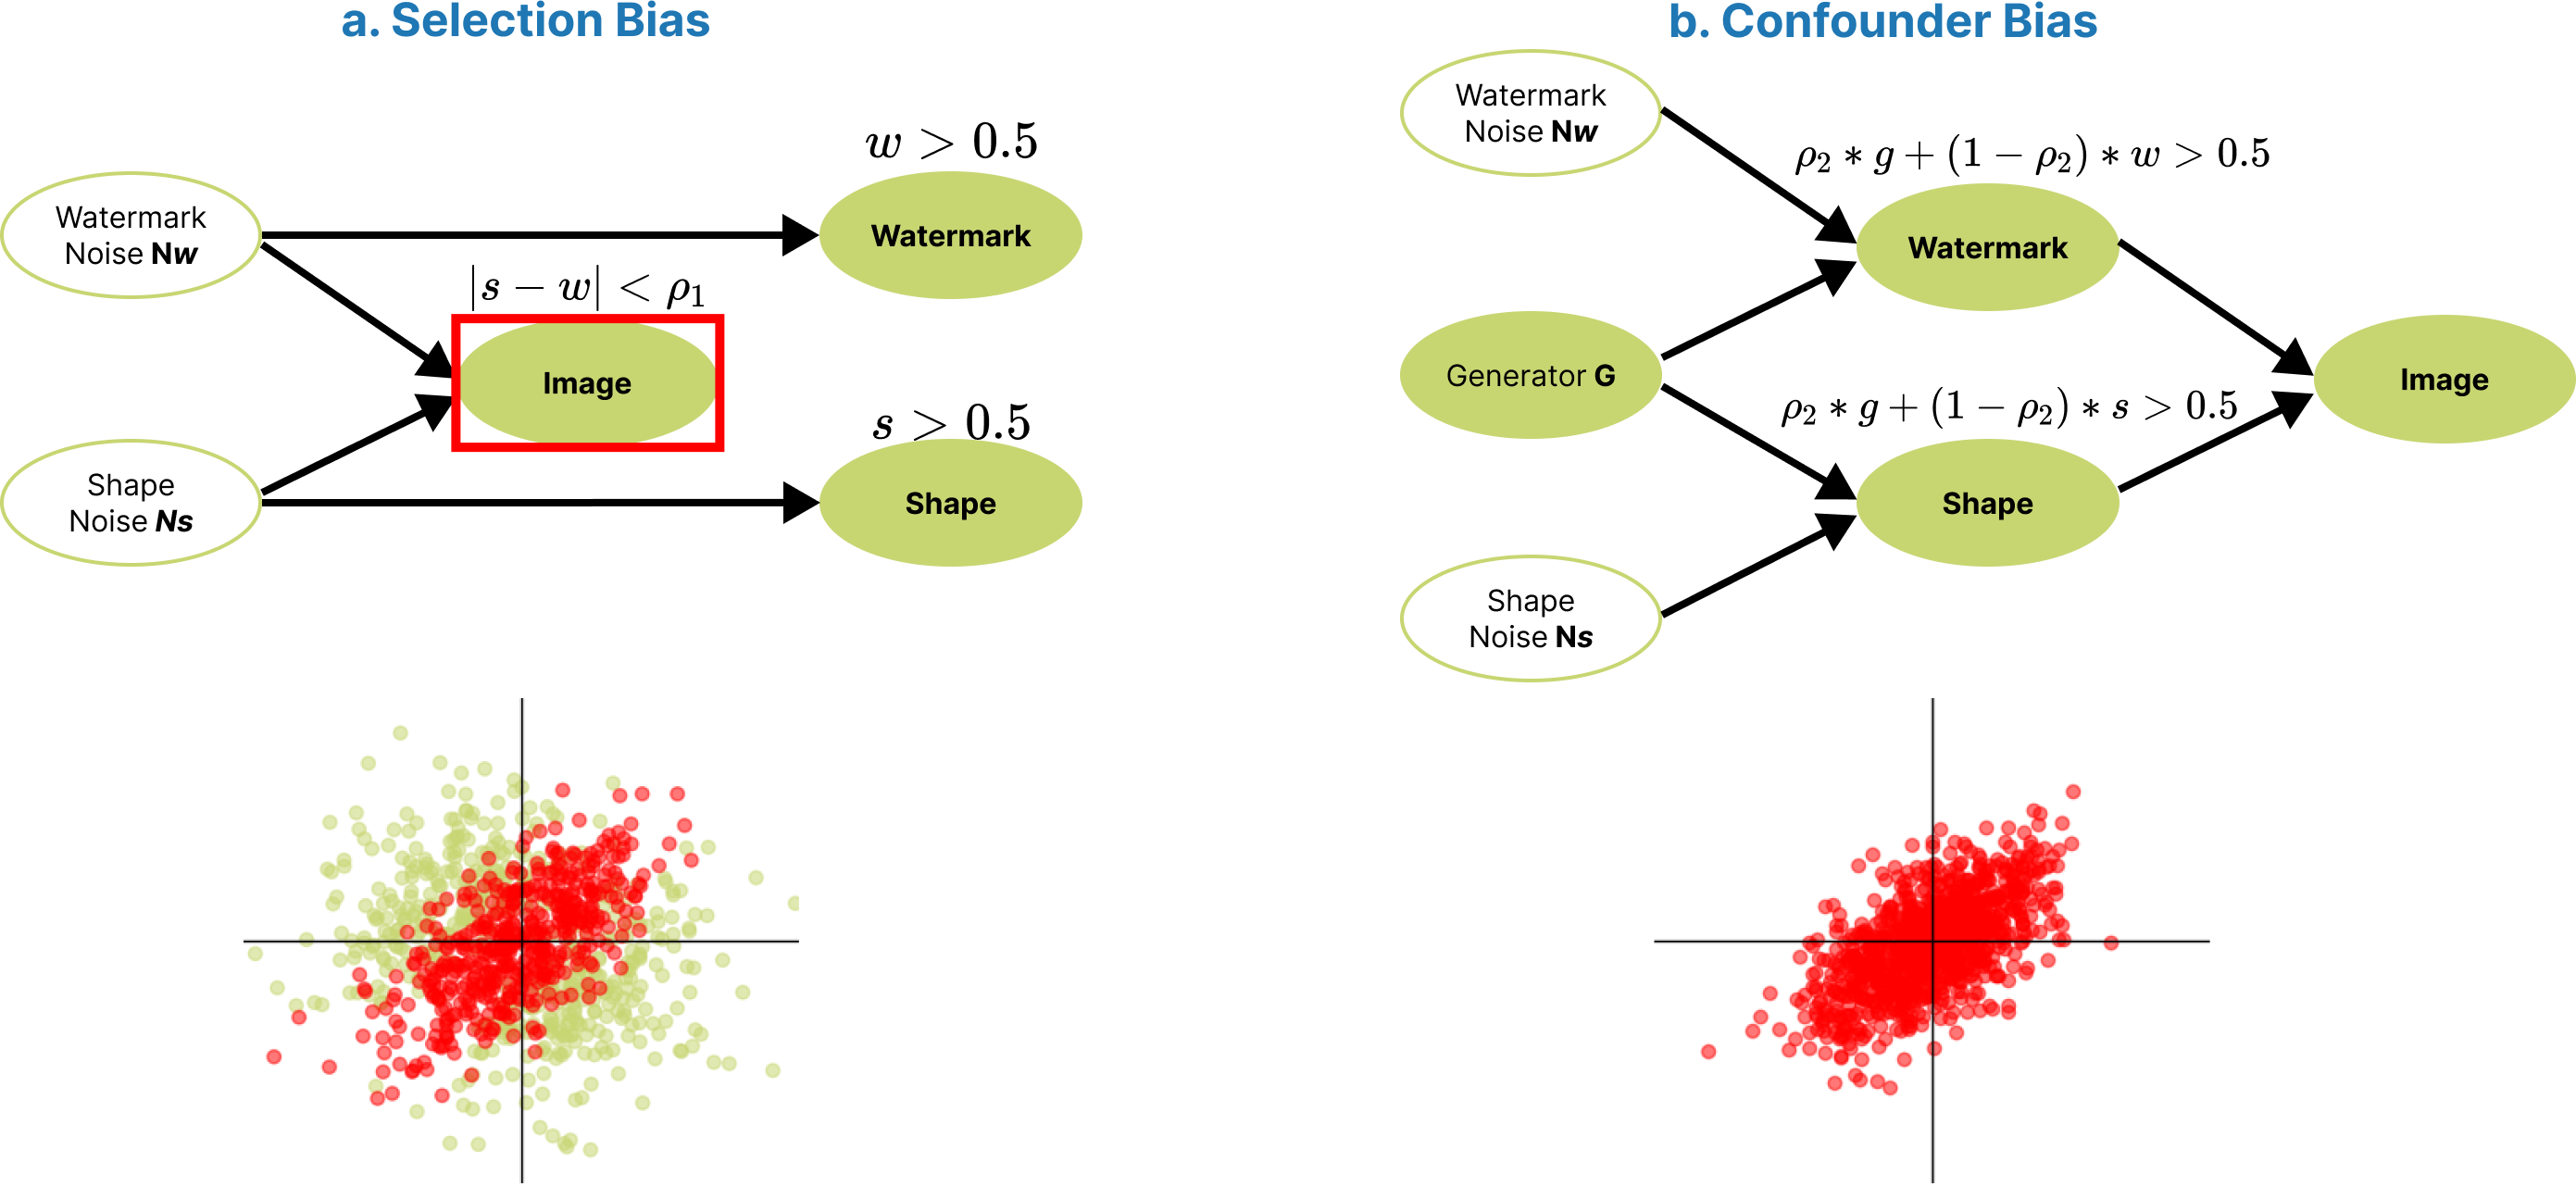
\includegraphics[width=0.8\textwidth]{pics/equivalent_scm.png}
    \caption[Selection vs. Confounder Bias]{SCMs typically found in image datasets.
    \textbf{a.} Selection Bias \textit{(researcher chooses images from free online collection with watermarks)}
    \textbf{b.} Confounder Bias \textit{(e.g. scientist marks positive x-ray scans with sign)}}
    \label{fig:equivalent_scm}
\end{figure}

\subsection{Explanation Generating Model}
The data generation causal model is part of the model which generates predictions and explanations.
This model is defined in a similar way to the \textit{explanation generating process (EGP)} in Karimi et al. \cite{Karimi2023}.
Ratio $\rho$ is a meta-variable of our image generation process in a similar sense to how hyperparameters are defined for the training there. While \cref{fig:generating_scm} depicts the data generating causal model (DGCM) of the training dataset in more detail, \cref{fig:egp} shows how this is embedded into the mechanism of generating explanations. 

\begin{figure}[H]
    \centering
    \tikzset{%
        neuron/.style={
                circle,
                draw,
                minimum size=8mm
            }
    }
    \begin{tikzpicture}[every node/.style={ draw, minimum size=8mm, align=center},]

    % generating model:
        \node [neuron]  (r) at (0.0,1) {$\rho$};
        \node [neuron]  (rs) at (0,2.5) {rand};
        \node [neuron]  (scm) at (2,1) {DGCM};
        \node [neuron]  (ws) at (5,2.5) {weights};
        \node [neuron]  (x) at (5,1) {$\mathcal{X}$};
        \node [neuron]  (p) at (7,2.5) {$Y$};
        \node [neuron]  (e) at (7,1) {$E$};

        \draw[->] (r) -- (scm);
        \draw[->] (rs) -- (ws);
        \draw[->] (scm) to (ws);
        \draw[->] (ws) -- (p);
        \draw[->] (x) -- (p);
        \draw[->] (x) -- (e);
        \draw[->] (p) -- (e);
        \draw[->, bend right=30, dotted] (r) to (e);
        
    % simplified causal model:
        \node [neuron]  (r) at (11,3) {$\rho$};
        \node [neuron]  (x) at (11,0) {$\mathcal{X}$};
        \node [neuron]  (p) at (13,1.5) {$Y$};
        \node [neuron]  (e) at (15,1.5) {$E$};

        \draw[->] (r) -- (p);
        \draw[->] (x) -- (p);
        \draw[->, bend right=30] (x) to (e);
        \draw[->] (p) -- (e);
        \draw[->, bend left=30] (r) to (e);
    \end{tikzpicture}
    \caption[Explanation Generation Process (EGP)]{Explanation Generation Process \textit{EGP} (left), Simplified Causal Model (right)}
    \label{fig:egp}
\end{figure}

\subsection{Watermark Benchmark Dataset W-dSprites}\label{section:causal_model}
Although this thesis is not the first work to use a toy dataset with known generating factors to evaluate attribution methods, we aim to find a new dataset which is as simple as possible and yet mirrors the main workings of a realistic computer vision problem. For this we adapted the dSprites dataset \cite{dsprites17} by adding small watermarks in the shape of '\textit{w}'s to some images. The dSprites dataset was originally constructed as a means for testing the degree of disentanglement a machine learning model has achieved. It contains images with rectangles, ellipses or hearts in varying positions, scales and rotations. To simplify the task more we only use the rectangle and ellipse class for our experiment. Another motive is that in a binary classification task positive and negative relevance might be used in varying strategies for prediction. In theory this could make the class-insensitivity studied by Sixt et al. \cite{Sixt2020} visible or counteract it. Further details can be found in the appendix \cref{appendix:dsprites}.

\begin{figure}[H]
    \centering
    \includegraphics[width=0.6\textwidth]{pics/dsprites_examples.png}
    \caption[Example Images W-dSprites]{First row: images from the original dSprites dataset, second row: images from the W-dSprites dataset with small \textit{w} as a watermark on some images in random positions at the edge of the image and Gaussian noise added.}
    \label{fig:dsprites_examples}
\end{figure}

\section{Generating Explanations with Concept Relevance Propagation}
The previously described causal framework can be applied to a multitude of explanation methods as it is principally model- and method-agnostic. However we limit our analysis to CRP and interpretation techniques constructed with CRP. This is mostly due to the time limitations of a master thesis, but also because they specifically claim in their paper to be able to identify relative importance using CRP. 
Producing explanations using concept relevance propagation requires decisions on the backpropagation rule(s), on the conditioning sets and further hyperparameters. 
We follow the recommendations and default settings of CRP's authors \cite{Achtibat2022, Achtibat2023} and best practices \cite{Kohlbrenner2020} as closely as possible.
For the backpropagation we apply the $LRP_{\varepsilon -z^+- b^-}$ - rule as recommended by \cite{Kohlbrenner2020}. Due to the simplicity of our CNN model no more model canonization steps need to be applied. See \cref{appendix:lrprules} for further technical details. 

\begin{figure}
    \centering
    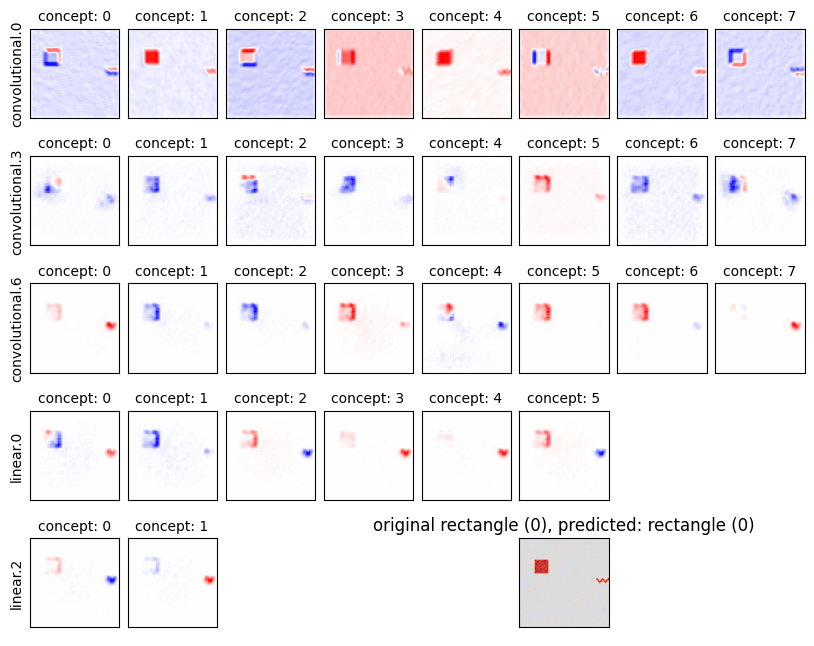
\includegraphics[width=0.8\textwidth]{thesis_latex_template/pics/conditional_heatmaps.png}
    \caption[Comparing Attribution Maps of Layers]{Concept-conditional heatmaps for one example image. Note the Sobel-filter-like attributions in earlier layers and the more combined attributions of watermark and shape in later layers.}
    \label{fig:cc_heatmaps}
\end{figure}

Principally, neurons in every layer of a model can be conditioned on using the CRP-approach. However, the resulting attribution maps are not necessarily depicting disentangled \textit{and} abstract enough concepts. When looking at \textit{concept-conditional} attribution maps from the earlier layers, one will likely see low-level features akin to Sobel-filter. In the late, fully connected layers before the output the previously disentangled concepts might get mixed together again for the final decision. In \cref{fig:cc_heatmaps} an example shows the tendency from trivial to abstract \textit{concepts}. 
According to \cite{Dreyer2023a} referring to \cite{Zeiler2013} the \textit{last convolutional layer} is ``most likely representing disentangled representation''. For comparison we investigate both the last convolutional and the first fully connected layer of the model. It is not entirely clear whether the extremely small size of our model hinders a transfer of the results to realistic scenarios. Yet, training significantly larger models would have been too computationally expensive for this principled approach, requiring many trained models.\\

In the following we will reiterate the steps necessary to produce the different components of CRP-explanations:

\subsubsection{Concept-Conditional Attribution Maps and Relevance for Prediction}
The concept-conditional backpropagation rule described in \cref{section:crp_background} can be applied to arbitrary sets of neurons (i.e. filters) $\theta$. In our scenario we create class-specific attribution maps conditioned on each neuron in the selected layer (last convolutional or first fully connected). For this we use the output for the ellipse class as the initialization for relevance, keep all other layers untouched and then itreatively mask out the other neurons relevance in the layer $\ell$. 
\begin{equation}
    R_{i}^{\ell}(\mathrm{x} |\theta_{\ell}=\{i\}) 
\end{equation}
Backpropagating all the way to the input yields an attribution map $R_i^{\ell}$, however the relevance $r_i$ assigned to the neuron in question from previous layers can be used as an approximation of its overall importance for the prediction.

\begin{itemize}
    \item should I keep class the same or change per instance?
    \item Should I really do everything both for last convolutional and first fully-connected layer?
\end{itemize}

\subsubsection{Local Concept Importance}
Masking the desired region in the image and computing attributions for this area. (is kinda the same as just taking importance in that area???, but then normalized with their recommended method)


{\color{gray} \subsubsection{Relevance Maximization}
To arrive at reference sets of the neurons in our selected layer, relevance maximization finds images that maximize concept-conditional relevance. As mentioned by \cite{Achtibat2022} using the whole dataset might make the selected images too similar to each other. Hence we compute the maximization for a subset of 1000 images to enforce more variance. Importantly, the sample we select from does not have the association between $S$ and $W$, meaning that watermarks are equally likely to occur on rectangle as on ellipse images. 
The implementation provided by CRPs authors produces sets of 40 images for each neuron in each layer. 

\subsubsection{Perceptive Field}
Information on the concentration of the relevance within the images selected for each concept can be gained by applying concept localization. Following the approach of \cite{Yeh2020} and using tools from the existing LRP toolset \cite{Anders2023} Achtibat et al. visualize only the part of the selected images that contributed to the neurons activation. 
The implementation of this and all previously described methods is made accessible by CRPs authors at \url{https://github.com/rachtibat/zennit-crp}.
}


\section{Data Ground Truth Correlation $m_0$}
The goal of this analysis it to gather information on how a known coupling ratio of two features interacts with their importance to the model and their explained importance. 
Measure $m_0 = \rho$ is the correlation between the shape and watermark feature in our data generating model. When $\rho$ is 0, the features are not associated at all, when it is 1 they correlate perfectly. Conceived as a \textit{signal-to-noise} ratio between the correlated and uncorrelated parts of $S$ and $W$, it can directly be used as a measure of the coupling of spurious (watermark) and core (shape) feature. However the data generating process introduces a small offset due to the binarization of the variables $W$ and $S$. It might therefore be more insightful to look at the actual correlation of the features in the generated data distribution as a ground-truth. This is also sensible because we only sample a small subset from the data generating SCM  for training and can not expect the distribution to perfectly align with $\rho$. Considering that we have two binary variables their correlation can be measured using the $\phi$-coefficient. It is also called \textit{Matthews} or \textit{Yule phi} coefficient and can be interpreted like the Pearson correlation coefficient for two binary variables:

\vspace{1em}
\begin{minipage}[t]{0.45\textwidth}
\begin{tabular}{|c|c|c|c|}
    \hline
     & y= 1 & y = 0 & total  \\  \hline
    x= 1 & $n_{11}$ & $n_{10}$ & $n_{1*}$ \\ \hline
    x= 0 & $n_{01}$ & $n_{00}$ & $n_{0*}$ \\ \hline
    total& $n_{*1}$ & $n_{*0}$ & $n$ \\ \hline
\end{tabular}
\end{minipage}%
\begin{minipage}[c]{0.45\textwidth}
\begin{align}
& \phi = \frac{n_{11} * n_{00} - n_{10}*n_{01}}{\sqrt{n_{1*}*n_{0*}*n_{*0}*n_{*1}}}
\end{align}
\end{minipage}
\vspace{1em}

Generally, we do not want and neither expect the model to perfectly reconstruct $\rho$ or the data correlation $\phi$. After all, the strength of neural networks presumably lies in recovering the truly important feature even when other, highly correlated features are present. Though some research expects explanations to give insight into the distributions of the training data to better understand how biases might occur, even if a model has apparently learned to ignore spurious features \cite{Kindermans2017}. 

\begin{figure}
    \centering
    \includegraphics[width=0.5\textwidth]{thesis_latex_template/pics/gt_m0_phi_only.png}
    \caption[Choosing measure for $m_0$]{$\rho$ plotted against $\phi$-coefficient of sampled training data distributions }
    \label{fig:finding_rho}
\end{figure}

\section{Establishing a Ground-Truth Model Feature Importance $m_1$}\label{section:gt_measure}
In contrast to realistic application scenarios our causal framework enables us to establish the ground truth importance of features for a trained model. Similar to recent work on causal attribution \cite{Goyal2019,Parafita2019,Karimi2023} the causal effect of an intervention upstream on the output of a model can be estimated in the following way:
\begin{center}
Average Causal Effect of latent factor $W$ on output $Y$ \\
\begin{equation}
\displaystyle ACE = \mathbb{E} [ Y \ | \ do(W=1) ] - \mathbb{E} [ Y \ | \ do(W=0) ] 
\end{equation}
\end{center}
The intervention on a given latent factor is straight-forward here, as our factors of interest are both binary variables (watermark and shape). Due to our knowledge of the ground truth we can condition on all other latent factors and feed one image with the watermark and the same image without it through the neural network. Thereby achieving a pure intervention on our $W$.  
However it is not naturally clear how to define the output of a neural network. One can either measure the average causal effect on the binary prediction or on the output layers' logits, which change in a continuous fashion.
To account for the effect of the initialization of model weights and biases on the usage of either feature, we average each measure over multiple random seeds (see \cref{fig:gt_over_seeds}).

\subsection{Prediction Flip}
Computing the Prediction Flip is straight forward in our example as we can control all variables. 
This binary causal effect can be estimated as the percentage of images for which the prediction flips, when the factor is flipped, which in turn is equivalent to the $\phi$-coefficient between prediction $Y$ and watermark $W$ (see proof in \cref{appendix:phi_equals_pf}). Therefore this measure is apt for the comparison with the $W,S$ correlation in the training data distribution.

We expect this variant of the model importance to only become sensitive to the spurious watermark feature $W$ for higher values of $\rho$. The reason being, that while the continuous output vector (i.e.\textit{confidence}) might already be affected by the spurious feature for weaker biases, the prediction will only flip once the spurious feature becomes more important than the core feature. For example, an image without a watermark might be correctly classified as an ellipse, but the same image with the watermark might have a higher activation for that class.

For better readability we will refer to an image with the watermark $\mathrm{x}_{do(W=1)}$ as $\mathrm{x}$ and the same image without the watermark $\mathrm{x}_{do(W=0)}$ as $\mathrm{x}'$ in the rest of the thesis.
\begin{align}
\displaystyle 
& PF =\frac{1}{|\mathcal{X}|} \sum_{\mathrm{x} \in \mathcal{X}} |y(\mathrm{x}) - y(\mathrm{x}') | \\
&  \equiv \frac{|\mathrm{x}_{W=1,y=1}|*|\mathrm{x}_{W=0,y=0}| - |\mathrm{x}_{W=1,y=0}|*|\mathrm{x}_{W=0,y=1}| }
{\sqrt{|\mathrm{x}_{y=1}|*|\mathrm{x}_{y=0}|*|\mathrm{x}_{W=1}|*|\mathrm{x}_{W=0}| }}
\end{align}


\subsection{Mean Logit Change}
For the W-dSprites classification task, the output vector consists of 2 logits $y_0$ and $y_1$. The model predicts \textit{rectangle} when $y_0 > y_1$ and \textit{ellipse} otherwise. To compute the mean logit change when intervening on our watermark spurious feature $x$, we take a sufficient amount of samples $\mathcal{X}$ from our dataset and feed them through the model. First we predict images with $W=1$ (containing a watermark) then with $W=0$. It is important to choose a reasonable distance measure between the two output vectors. \cite{Sixt2022a} and \cite{Goyal2019} use the mean absolute difference (or $L1$-norm). To enable better comparison we use the soft-max confidences as during the training process. This keeps the relative magnitudes within the sample set intact but brings it to the range $[0,1]$. All measures are scaled so that the distance for maximally different instances is 1, which in this case means dividing by 2. Although we compute the euclidean distance for the explanations later, this is not necessary here, as for 2D vectors $D_{euclid} = \sqrt{D_{abs}}$.\\

Mean Absolute Difference:
\begin{align}\displaystyle 
& \MLC_{\rho, m}^{abs} = \frac{1}{|\mathcal{X}| * 2} \sum_{\mathrm{x} \in \mathcal{X}} 
|y_0(\mathrm{x}) -y_0(\mathrm{x}')| + |y_1(\mathrm{x}) -y_1(\mathrm{x}')| 
\end{align}

Recently, assessing the similarity of activation and relevance vectors has been done using the cosine similarity \cite{Sixt2020, Dreyer2023a, Achtibat2022}. Therefore we also include the cosine distance as a potential distance metric for the model output (as well as the explanation later). We are not convinced that this measure has properties we seek for evaluating logits of a network as it does not exhibit triangle inequality. However it seems useful to incorporate metrics used by other authors to enable comparison. Through the soft-max scaling of the output confidences we can nevertheless ensure the magnitude to not be ignored by this measure, which can be interpreted as angular dissimilarity. Without that the cosine distance of e.g. $[-0.5,0.5]$ and $[-10,10]$ would be 0, but for their soft-maxed counterparts the resulting distance is $0.06$. \\

Cosine Distance:
\begin{align}\displaystyle 
& \MLC_{\rho, m}^{cosine} = \frac{1}{|\mathcal{X}|}\sum_{\mathrm{x} \in \mathcal{X}}  
1 - \frac{\vec{y}(\mathrm{x}) \cdot \vec{y}(\mathrm{x}')}
{\lVert \vec{y}(\mathrm{x}) \rVert \lVert \vec{y}(\mathrm{x}')\rVert }
\end{align}


\section{CRP Explanation Importance $m_2$}\label{section:measure}
Our goal is to compare the causal effect of an upstream intervention on the true feature importance and then the explained feature importance. After having defined multiple ways to measure the models true feature importance, we need to repeat the process for the concept-based explanation produced by CRP. It is not well known how humans perceive changes in an explanation and there is no agreed upon scale of importance, so we believe it is best to construct multiple measures to test against each other. Most of the proposed metrics are derived from existing work on evaluating feature importance in XAI \cite{Sixt2020, Karimi2023, Arras2022} 
 {\color{gray} Additionally, the authors of CRP introduce multiple interpretation techniques using this method which potentially enable better human understanding. }\\

Each candidate should be a variation of measuring the effect of intervening on $W$ on an explanation:
\begin{center}
Average Causal Effect of latent factor $W$ on explanation $e$: \\
\begin{equation}
\displaystyle ACE = \mathbb{E} [e \ | \ do(W=1) ] - \mathbb{E} [ e \ | \ do(W=0) ]
\end{equation}
\end{center}
The core question is, whether the influence on the explanation of changing $\rho$ is completely mediated by our prediction. A perfect explanation assigns just as much importance to a feature as the model and does not depend on other factors. This is one way to describe the fidelity of the explanation to the model. The proposed measures however partly incorporate other notions of goodness applied for XAI such as \textit{complexity}. This also has the practical reason that while an attribution map is visually compelling, it is not a very concise description of relevance. At least in the case where ground-truth concepts are known, we can estimate the explanation importance in a more compact form. \\

The measures introduced in the following are roughly ordered from measures being most true to the numerical effect of intervention on the explanation to measures reducing the complexity of the explanation. Although human perception is not part of our evaluation, aiming for less complex explanations seems to be more in line with a \textit{good} explanation. While the first measure would require a pixel-wise comparison of multiple heatmaps to find differences, later metrics try to use only one pixel or a reduced (hopefully more human-understandable) concept. \\

Many related works remove negative relevances in attribution maps to enable comparison with XAI methods that do not measure negative relevance. Another reason could be that incautious aggregation of attribution maps with negative and positive relevance could introduce cancelling-out effects. We believe, however, that a spurious feature can be negatively as well as positively attributed for a model to be biased. In a complex network, we cannot be sure that there are no neurons purely negatively associating a feature with one class. Therefore the measures mostly equally incorporate both the magnitude of the positive and negative relevance. 

\subsection{Mean Attribution Change}
The likely most straight-forward way to calculate explanation importance for neurons in a layer using CRP is to measure the average causal effect of an intervention on the attributions directly. This approach aims to emulate the \textit{mean logit change} of the prediction for the concept-based explanation. In a given layer $\ell \in L$, the relevance of each of the neurons $i in \ell$ for the overall prediction is used. As in \cite{Achtibat2022}, the relevances for the neurons are scaled to sum to 1 and are interpreted as relative importance percentages.
Also, the attributions for each of the $|\ell|$ neurons in $|\ell|$ concept-conditional heatmaps is computed using CRP.

We compute the neurons relevance and their attribution map with the CRP method the following way:
\begin{align*}
& r_i(\mathrm{x}) = R(i | \theta=\{y\}) \\
& R_i^{\ell}(\mathrm{x}) = R(\mathrm{x} | \theta=\{i, y\}) \\
\end{align*}

The causal effect of intervening on the spurious watermark feature on one neuron is then the difference between its attribution map of one image with a watermark and the same image without a watermark. If the model has indeed learned distinct concepts for each feature, the same effect should also become visible, when just looking at the relevance values for each neuron in a layer.\\

To look at the difference in explanation, multiple distance metrics could be applied. We compare multiple types of dissimilarity between the two heatmaps (i.e. 2-dimensional pixel maps). Firstly, we look at the mean absolute pixel-wise difference. The Euclidean distance seems the second natural approach. Because we compute the \textit{cosine distance} for the relevance values $r_i$ as proposed by the authors of CRP \cite{Achtibat2023}, we also compute the measure for the attribution maps for completeness.
Lastly, we measure the kernelized treatment effect which Karimi et al. also use in their experiment \cite{Karimi2023}. It is using a 2D convolution to multiple images. For 1 dimensional vectors like the predictions and the relevances, this corresponds to a simple dot product.   \\ 

A sensible normalization for a set of attribution maps is not as trivial as for the output vector or the relevance vector. The naive approach would be again, to take the maximally opposing images difference. But it is not to be expected that any method would assign large positive or negative values to every pixel. Instead, the results of attribution methods only sparsely assign attribution to few pixels, usually within regions of objects and not to the background. 
We therefore have to find a smaller divisor which scales a maximal difference between an image with and without watermark to approximately 1.
To adjust for the sparsity of the attributions, we take the maximal sum of absolute values of all heatmaps sampled for one model. This \textit{maximal absolute sum} scaling is similar to what Achtibat et al. \cite{Achtibat2022} apply to the relevances of a layer to interpret them as (positive or negative) percentage values.\\

Here we show the different possible distance metrics for the attribution maps.
\begin{align}
\displaystyle 
& r_{tot}(\mathrm{x}) = \sum_{i \in \ell} \sum_{p \in P_x} 
|R_{p,i}(\mathrm{x})| \notag \\
& \max_{\rho, m}^E = \max_{\mathrm{x} \in \mathcal{X}} (r_{tot}(\mathrm{x}) , \  r_{tot}(\mathrm{x}') ) \notag \\
& \MAC_{\rho, m, \mathrm{x}}^{abs} = 
\sum_{i \in \ell} \sum_{p \in P_x} |R_{p,i}(\mathrm{x}) -R_{p,i}(\mathrm{x}')|* \frac{1}{\max_{\rho, m}^E} \\
& \MAC_{\rho, m, \mathrm{x}}^{euclid} = \sqrt{ \sum_{i \in \ell} 
\sum_{p \in P_x}\left(\frac{R_{p,i}(\mathrm{x}) -R_{p,i}(\mathrm{x}')}{\max_{\rho, m}^E}\right)^2
} \\
& \MAC_{\rho, m,\mathrm{x}}^{cosine} =
\frac{R(\mathrm{x}) \cdot R(\mathrm{x}') }{|R(\mathrm{x})|\cdot |R(\mathrm{x}')|} \\
& \MAC_{\rho, m, \mathrm{x}}^{kernel} = k(R(x) ,R(x) ) + 2 k(R(x) ,R(x') ) + k(R(x') ,R(x') )  
\end{align}

Once a distance metric is chosen, we need to aggregate results over all sample images, and then again over the models initialized with different seeds.

\begin{align}
& \frac{1}{|M_\rho|\cdot |\mathcal{X}| }\sum_{m}^{M_{\rho}} \sum_{\mathrm{x,x'}}^{\mathcal{X}} Metric(\mathrm{x,x'})
\end{align}

The pixel-wise relevance should be assigned to different attribution maps proportionally to the total relevance over the different neurons of the layer, but it might still be reasonable to weigh the per-neuron distance with its absolute relevance $r_i$. The reason being, that high variation in unused or unimportant neurons might distort the overall distance, while there are less differences in the important pixels and vice-versa:

\begin{align}
& \frac{1}{|M_\rho|\cdot |\mathcal{X}| }\sum_{m}^{M_{\rho}} \sum_{\mathrm{x,x'}}^{\mathcal{X}} \sum_{i in \ell} 
Metric(\mathrm{x,x'}, i) * |r_i(\mathrm{x})|
\end{align}

Although this (possibly weighted) difference is constructed to measure the causal effect of intervention on the explanation as closely as possible, it ignores one of the core ideas of concept-based and local attribution methods potential usefulness. If adding or removing a watermark has a significant effect on some pixels far away from it, this is not in line with desirable properties of a good explanation such as interpretability or even fidelity to the ground truth importance. It is likely that through the coupling of watermark and shape in our experiment, the changes of relevance do not only affect the watermark region itself but at least the shapes importance too. 
Another potential downfall for human intuition is the way more localized concepts are attributed in comparison to more global or wide-spread concepts. Achtibat et al. \cite{Achtibat2022} show an example where the eye of a dog wrongly seems to be more important than its fur in a general attribution map, because it is concentrated on a smaller region. A similar thing can potentially happen with our experiments watermark, as it fills a small region in comparison to the larger shape feature. 

In the \cref{section:region_specific} we thus introduce measures which concentrate on the attributed relevance within the ground-truth region and relative to the rest of the attribution map.
We also further reduce the estimation of whether a concept (i.e. filter) encodes the spurious watermark feature or something else. 

\subsection{Concept Relevance Vectors}
Without looking at the attribution maps it is still interesting to see whether the total relevance of certain neurons changes when intervening on the watermark $W$ or the shape $S$ feature. If the neural network indeed follows different strategies when the watermark is present versus when it is not, then different concepts should be relevant depending on the features value. 
In contrast to previous measures, this measure is not computed in the attribution map space, but only in the relevance space. We therefore have no information on which concepts the filters encode, only how important they are. Achtibat et al. still look at concept relevances extensively as they assume them to encode human-understandable concepts. While for the previous measures the aim was to extract the importance from the visual explanation, for this measure we only assume that different filters should be at work depending on the presence of the watermark, if it has significance.
We find it necessary to make this distinction: A filter could change strongly when intervening on the watermark. But if this change (or the importance of the watermark for that filter) is not visible from the attribution maps, it is impossible to decipher which concept that filter encodes without access to ground-truth concepts. 

For the relevances within a layer, we apply the same distance metrics as described in the previous section except that summing over pixels is not necessary. Also, the relevances are already in a $[-1,1]$ interval and sum up to maximally 1 per image due to the recommended normalization. The resulting distances however can range up to 2 because of possible negative relevances, hence we divide the effect sizes by 2 to facilitate comparison. 

\subsection{Importance in Ground-Truth Region}\label{section:region_specific}
In \cite{Arras2022} two metrics for the analysis of importance in pixel maps are introduced. Relevance Mass Accuracy (RMA) measures the ratio of relevance within a bounding box around a feature to the total relevance. Relevance Rank Accuracy (RRA) rates the percentage of pixels in such a bounding box that fall within the $k$ most important pixels in the heatmap. If those metrics are accurately describing the relative importance of a feature for the explanation too, they should be applicable in our experiment. 

\subsubsection{Relevance Mass Accuracy (RMA)}
When trying to establish whether a feature is important, one would intuitively look at that feature first. Therefore approaches like Relevance Mass Accuracy take into account the known boundary of a feature for benchmarks with ground-truth importance. Luckily, in our benchmark dataset the shape and watermark feature are spatially separated so this strategy is applicable.
Bau et al. \cite{Bau2017, Bau2020} have defined a similar measure to compare an explanation importance to a ground truth, which they term IoU (from \textit{Intersection over Union}). Both these works assume the perfect attribution of importance to one feature to be a binary mask, which is 1 inside and 0 outside the features region. \\
As noted in \cite{Arras2022} it is not known whether this perfect score is attainable or even desirable for an explanation. Yet the overall tendency should become clear.

For our localized metric we apply a strategy resembling these evaluation scores. 
Fortunately, the authors of CRP have already formulated \textit{local concept importance}, evaluating the conditional attribution to a concept in a predefined region by masking the rest of the attribution map out. 
While RMA in the CLEVR-XAI benchmark uses the exact pixel-boundary of an object, we use a bounding box around the watermark \textit{w}. This is because the small model we apply smoothes out relevance over a region due to pooling layers in the model. \\

\begin{figure}
\begin{minipage}[t]{0.45\textwidth}
    \vspace{-\topskip}
        \includegraphics[width=\textwidth]{thesis_latex_template/pics/bounding_box.png}
\end{minipage}
\begin{minipage}[t]{0.45\textwidth}
    \begin{align}\displaystyle
    & R_B(\mathrm{x}) = \sum_{p_x \in B} R_{p_x}(\mathrm{x} | \theta)\\
    & RMA(\mathrm{x}) = \frac{R_B(\mathrm{x})}{R(\mathrm{x})}
    \end{align}
\end{minipage}
\caption{Bounding Box $B$ around watermark}
\label{fig:bounding_box}
\end{figure}

The \textit{localized relevance score} is the amount of conditional relevance attributed to a certain region of an image. In our case, the region of interest are pixels in the bounding box $B$ around the watermark (see \cref{fig:bounding_box}. 

To enable better comparison we again embed this measure within the watermark/no watermark effect estimation setting, even though we do not expect an image without a watermark to apply any relevance within the bounding box.

Albeit this approach is reducing complexity, it has been noted that importance is hard to gauge when features have varying spatial extends. \cite{Achtibat2022} points to an example where the fur of a dog actually has larger total relevance but in the heatmap the snout seems to be more important because its attribution is more concentrated. A similar thing could happen with the watermark feature because it is usually smaller than the shape itself. 
To potentially combat this, we set the relevance within the bounding box in relation to the total relevance, which yields the RMA score.
While this metric might give us a good estimate of the actual relevance of the watermark, the heatmap could still produce a wrong understanding of relative relevance for humans. \\

\subsubsection{Relevance Rank Accuracy (RRA)}
The second metric adapted from \cite{Arras2022} is \textit{Relevance Rank Accuracy}.  
Relevance Rank Accuracy orders the input features (i.e. pixels) by relevance and finds the $k$ most relevant pixels. The rank $k$ is equal to the size of the region of the feature, in question, here the bounding box around the watermark. Computing the ratio of the top-k relevant pixels inside of the bounding box $B$ to $k$ yields \textit{Relevance Rank Accuracy}:

\begin{align*}
& P_{top-k} = (p_1, p_2,...,p_k | |R_{p_1}| > |R_{p_2}| > ... > |R_{p_k}| ) \\
& RRA(\mathrm{x}) = \frac{|P_{top-k} \cap B|_\mathrm{x}}{|B|} 
\end{align*}

Arguably, this metric loses even more information on whether at least some importance is assigned to the spurious feature (watermark). Previous work has also pointed out many issues with this or similar methods. However it reduces the complexity of the explanation by only looking at the k-most important pixels. \\

\subsubsection{Pointing Game}
A step towards even more reduced complexity is the \textit{Pointing Game} metric, first introduced in \cite{Zhang2016}. The only difference between RRA and the Pointing Game metric is, that the latter \textit{binarizes} the question whether a feature is important by setting $k = 1$. If the most important pixel is inside the watermark bounding box $B$, the watermark is important, otherwise not.
We can then use this information as a binary weight on the relevances of concepts. 
It has been noted by others that the pointing game metric is sub-optimal for evaluating attribution maps, as pointing to the central pixel in an image already produces ''good'' results. However, as our watermark changes position on the sides of the image and is quite localized, we think that this measure can still function as an approximation. 

These metrics are all defined for one general heatmap and we have to find a generalization for $|\ell|$ attribution maps for the filters in a layer. Just summing up the values for all concepts would not generate a useful result as the relative relevance of each filter is removed from these region-specific measures. Instead, we create a weighted sum of the scores over the neurons. As weights we use the absolute relevances $|r_i|$ to potentially incorporate negative relevance of the spurious feature too. 

\section{Direct vs. Indirect Influence of $\rho$}
After having computed a ground truth effect of $m_0 = \rho$ on the feature importance (of the watermark feature $W$) and the effect on the explanation, we can compare them.
While a visual comparison of the curves of importance might award us a first impression, measures like mutual information, correlation can be applied to give us real insights. 
In general it is not clear which type of relationship (linear, non-linear) to expect between $m_0, m_1, $ and $m_2$. Therefore the methods we can apply to test the independence of $E$ on $\rho$ given $Y$ are only an approximation and not definite.

\begin{figure}
    \centering
    \includegraphics[width=0.8\textwidth]{thesis_latex_template/pics/gt_m0_m1.png}
    \caption[$m_0$ vs. $m_1$]{Comparing $\phi$-correlation coefficient (blue) and mutual information (MI) (red) between shape and watermark for subset of 6400 images. \\ \textit{dashed}: true label biased data distribution, \textit{dotted}: prediction for biased data distribution \textit{solid}: prediction for unbiased data distribution }
    \label{fig:m0_m1}
\end{figure}

In \cref{fig:m0_m1} the relationship between our causal variable and the coupling within the datasets becomes visible, while the relationship to what the model has learned is not as \textit{linear}. The most concerning result would be, if the explanation had an even weaker relationship with $\rho$ than the prediction. That would be mean that the explanation is not able to recover spurious features sufficiently. 

Here we need to expand on exactly which methods we apply to compare the effects on prediction vs explanation. 

Karimi: Compare effect of Rho on Y and Rho on E with correlation analysis. Then randomly permute predictions Y, Compute Explanations E thereof. Again perform correlation analysis Rho,Y,E. 
use performance buckets with control group either within each performance bucket or use same accross all buckets. 
We have to do it differently here.

Easiest: 
- MSE or similar distance metric
- correlation (Pearson???)
- something that encodes correlation but penalizes, if measures scales differ to strongly (i.e. they increase proportionally, but the one reaches 1, the other only 0.2)


\section{CNN Model Zoo}\label{section:training}
To evaluate explanations, the model to test on can neither be to simple and therefore easy to explain, nor too large and therefore an overkill for the simple dataset at hand.
Through a simple trial-and-error search the architecture detailed in \autoref{lst:cnnmodel} with 3 convolutional layers of 8 channels, one fully connected \textit{concept} layer with 6 neurons and finally the fully connected output layer was deemed most fitting for the task. While less convolutional channels or layers often resulted in the model not converging at all, having more neurons or potentially \textit{concepts} did not seem to add information but just redundancy.
This model reliably yields test accuracies over 90\% when using the same feature distribution $\rho$ as used for training. As stated before, we fix all hyperparameters, as they are not part of this analysis, to values produced from a short search.
The only hyperparameter we deemed necessary to control for, is the random initialization of weights and biases. In preliminary experiments it became clear that some seeds react profoundly differently to $\rho$ than others. For example, one instance is able to ignore the watermark even when it is perfectly correlated with the shape ($\rho = 1$), while others easily change their strategy to predict from this spurious feature (see \cref{fig:gt_over_seeds}). This ground-truth importance and the general performance of the models seem to not correlate with each other. For example seed 0 produces similarly high accuracies as seed 3, while their reaction to the spurious feature is completely different. Therefore it is right to keep those \textit{unbiased} models in the set of models and not exclude them. 
For further information on hyperparameters and training, refer to \cref{appendix:model}.

\begin{figure}
    \centering
    \includegraphics[width=\textwidth]{thesis_latex_template/pics/compare_seeds_w_accuracy.png}
    \caption[Comparing Seeds]{Prediction Flip ($\phi$-coefficient between prediction and watermark) over 16 random seeds (red)
    compared to $\rho$ (green dashed), mutual information in distribution (blue dash-dotted) and training accuracy (gray dotted).
    }
    \label{fig:gt_over_seeds}
\end{figure}

{\color{codepurple} 
\textbf{Notation}:
\begin{enumerate}
    \item Image instances $:= \mathcal{X}$, one image $:= \mathrm{x}$
    \item pixels in image $\mathcal{X} := p_x$
    \item Watermark variable $:= W$ value for variable $:= w$
    \item bounding box of watermark $:= B$
    \item Shape variable/ label $:= S$ value for shape $:= s$
    \item coupling ratio $:= \rho$
    \item prediction $:= P$
    \item explanation variable $:= E$ single instance of explanation $:= e$
    \item Layer set $:= L$, Layer in neural Network $:= \ell$ neuron in layer $:= i$
    \item other factors $:= Z$ single factor $:z_i$ \\ 
    \textit{enumerate: scale, rotation, posX, posY}
    \item (Gaussian) noise terms for each causal var $:= N_{variable}$
    \item Random Seed number $:= M (=10)$, one seed/ index $:=m$
\end{enumerate}
}
\chapter{Experimental Results}\label{chapter:results}

{ \color{red}
10-20 pages 

    \begin{itemize}
        \item (1/3 of thesis)
        \item whatever you have done, you must comment it, compare it to other systems, evaluate it
        \item usually, adequate graphs help to show the benefits of your approach
        \item caution: each result/graph must be discussed! what's the reason for this peak or why have you observed this effect
    \end{itemize}
}


\section{Experiments}
\begin{itemize}
    \item what have I tried out with the different methods?
    \item list in concise order the possible measures
    \item ground-truth feature importance: mean logit change for output, R2-score,  prediction flip
    \item baseline explanation feature importance - thats what we compare to e.g. watermark bounding-box importance for summary heatmap
    \item special concept explanations feature importance
    \item how are the experiments set up, how do i make sure they are all well comparable
    \item to which other baseline could my measures be compared to?
\end{itemize}

\section{Results}
lots of plots!
\begin{itemize}
    \item what have I tried out with the different methods?
    \item what works and what doesn't
    \item plot for each experiment/possible method?
          \begin{itemize}
              \item watermark bounding box average relevance for different subgroups, somehow get difference
              \item variance of latent factors in relevance maximization image set - low variance means it encodes the concept
              \item naive: total relevance for watermark image region
              \item total activation + relevance of neuron given just watermark image
              \item one idea: take masked/bounding box approach again for neurons individual heatmaps
              \item nmf idea: somehow try to reduce the latent space to Watermark/Shape axis and measure variance in either direction
              \item centroids idea: use random DR algorithm and calculate ratio of centroid distances (needs latent factors again)
              \item causal idea??? somehow measure causal effect? - the other things are kind of causal or?
          \end{itemize}
\end{itemize}



\section{Evaluation}
\begin{itemize}
    \item evaluation of evaluation criteria:
    \begin{itemize}
        \item takes into consideration the whole latent space spanned by the concepts
        \item orients itself on known human cognition, user studies in this field would suggest this??? 
        \item performs similar to baseline watermark bounding box importance? 
        \item ...? \todo{define success criteria of finding a good measure}
    \end{itemize}
    \item which measure is the best according to those criteria
    \item which measure is the closest to ground truth
    \item which is the furthest from ground truth
    \item does measure find \textit{more information} than CRP itself and could possibly be used as a method on top of CRP for disentanglement/ spurious-core relation explanation?
    \item 
\end{itemize}

\section{Verification on Other Well-Known Benchmarks}
\todo{should i do this? which benchmarks, how to setup causal model for them etc. }
\begin{enumerate}
    \item Test method on more complex dataset e.g. CLEVR-XAI
    \item compare CRP to other XAI methods?
\end{enumerate}

\section{Discussion}
\begin{itemize}
    \item do measures work
    \item what does causality help us with
    \item is CRP better for constant vector shift stuff or does it still suffer from it?
    \item can the application of those measures further explain/inform the explanation?
    \item what failed miserably
\end{itemize}

\chapter{Conclusion}\label{chapter:conclusion}

{ \color{red}
    \begin{itemize}
        \item (1 page)
        \item summarize again what your paper did, but now emphasize more the results, and comparisons.
        \item write conclusions that can be drawn from the results found and the discussion presented in the paper.
        \item future work (be very brief, explain what, but not much how)
    \end{itemize}
}
\begin{enumerate}
    \item which ground-truth feature importance measure is best
    \item interesting points looking at model performances and explanation perforcmance?
    \item baseline vs. concept metric, which one is better for CRP
    \item performance on other cases
    \item how has causality helped in this?
    \item Answer Question: \textit{ARE WE EXPLAINING THE DATA OR THE MODEL} \todo{answer question}
\end{enumerate}

\section*{Limitations and Future Work}


{ \color{red}
    \begin{itemize}
        \item max 1-2 pages, could also be included into the conclusion section 
    \end{itemize}
}

%---------------------------------------------------
%----- Bibliography
%---------------------------------------------------
\addcontentsline{toc}{chapter}{References}
\renewcommand\bibname{References}
\bibliographystyle{acm}
\bibliography{bibdata.bib}


%---------------------------------------------------
%----- Appendix   
%---------------------------------------------------
%\backmatter
\appendix
\chapter{Appendix}\label{chapter:Appendix}


\section{Additional Details to LRP Rules and CRP Implementation}
\label{appendix:lrprules}
\begin{figure}[ht]
	\centering
	\label{fig:tesfigure}
	\includegraphics[width=\textwidth]{pics/test.png}
	\caption[Test Figure]{This is a test figure}
\end{figure}
\begin{itemize}
    \item explain used LRP rule \textit{epsilon plus flat} in sufficient detail
    \item explain what canonizers are and why they are not necessary for my example (model is simple and does not have batch norm layers) 
\end{itemize}


\section{Details on Adapted dSprites Dataset}\label{appendix:dsprites}
Has 737280 64x64 pixel binary images, only take rectangles and ellipses (Heart is to easy to distinguish?). so 419.. images.

The generating factors \verb|shape|, \verb|scale|, \verb|rotation|, \verb|x position| and \verb|y position| are known for each sample.

To adapt the benchmark for our purpose, only the first two shape classes (rectangle and ellipse) are used. A watermark in the form of a small \textit{w} was initially added to the lower-left corner of some images. During initial testing with only these adaptations it became clear that even the small convolutional neural network employed here is too powerful for this task as effectively dividing the image into two parts solves the problem and most neurons became irrelevant.
To make the spurious feature, which is the watermark \textit{w} more difficult to learn, its position is therefore varied across the edges of the image. Further a small uniform noise term is added to make the problem more realistic and the saliency maps more convincing and informative.
The aim of this new dataset is, to create the simplest possible scenario with known generating factors, while keeping it as realistic or close to real world application cases of attribution methods as possible. In \autoref{fig:dsprites_examples} the resulting images are visualized.


\todo{why the heck new dataset???}
\begin{itemize}
    \item why do we need another dataset for benchmarking watermark bias??
    \item some other benchmarks that deal with similar questions are...
    \item why am i not just using 3d shapes dataset? \url{https://github.com/deepmind/3dshapes-dataset/} (C. Burgess and H. Kim)
\end{itemize}


\section{Proof $\phi$-Coefficient is equal to Prediction Flip}
\label{appendix:phi_equals_pf}
\begin{table}[t]
    \centering
\newlength{\width}
\width15mm
\begin{tabular}{|c|c|c|c|c|c|}
    \hline
     \multirow{2}{\width}{}& \multicolumn{2}{|c|}{w=1} &\multicolumn{2}{|c|}{w=0} & \multirow{2}{\width}{total}  \\  \cline{2-5}
     & x=1 & x= 0 & x= 1& x= 0 &\\ \hline
    \multirow{2}{\width}{y= 1} & A $n_{111}$ & B $n_{110}$& C $n_{101}$& D $n_{100}$&\multirow{2}{\width}{$n_{1**}$}    \\ \cline{2-5}
    & \multicolumn{2}{|c|}{$n_{11*}$ }& \multicolumn{2}{|c|}{$n_{10*}$} &  \\ \hline 
    \multirow{2}{\width}{y= 0} & E $n_{011}$& F $n_{010}$& G $n_{001}$& H $n_{000}$& \multirow{2}{\width}{ $n_{0**}$} \\ \cline{2-5}
    & \multicolumn{2}{|c|}{$n_{01*}$} & \multicolumn{2}{|c|}{$n_{00*}$} & \\ \hline 
    \multirow{2}{\width}{total} & $n_{*11}$&  $n_{*10}$&  $n_{*01}$&$n_{*00}$& \multirow{2}{\width}{ $n$ } \\ \cline{2-5}
    & \multicolumn{2}{|c|}{$n_{*1*}$} & \multicolumn{2}{|c|}{$n_{*0*}$} & \\ \hline
\end{tabular}
    \caption{Caption}
    \label{tab:tBLE}
\end{table}

\begin{align*}
\phi = \frac{n_{11*} * n_{00*} - n_{10*}*n_{01*}}{\sqrt{n_{1**}*n_{0**}*n_{*0*}*n_{*1*}}} 
& PF = \frac{X}{n_{*0*}+n_{*1*}}
\end{align*}


\section{Model, Hyperparameters and Training}\label{appendix:model}
\subsection{Model Architecture}
For our analysis we decided on a model architecture that is small enough to train a few hundred times but big enough to still have high performance and be comparable to the deep neural networks that local attribution methods are typically applied to.
We deemed 3 convolutional layer and one fully connected layer before the final output layer enough for our task. Notably, the layers have comparably few channels (8 or 6). The objective of creating such a narrow network was to be able to visually compare \textit{all} filters within a layer in order to identify the human-understandable concepts they potentially learned. 

\begin{lstlisting}[language=bash, label=lst:cnnmodel]

convolutional_layers: 
    0: Conv2d(in_channels=1, out_channels=8, kernel_size=3)
    1: MaxPool2d(kernel_size=2, stride=2)
    2: ReLU()
    3: Conv2d(in_channels=8, out_channels=8, kernel_size=5)
    4: MaxPool2d(kernel_size=2, stride=2)
    5: ReLU()
    6: Conv2d(in_channels=8, out_channels=8, kernel_size=7)
    7: ReLU()

linear_layers:
    0: Linear(in_features=392, out_features=6, bias=True)
    1: ReLU()
    2: Linear(in_features=6, out_features=2, bias=True)  

\end{lstlisting}

\subsection{Hyperparameter Choice}
The values for hyperparameters of the training process are optimized for accuracy with a rather short search. Finally, we train all models using the \verb|Adam| optimizer with a learning rate of \verb|0.001| using \verb|cross-entropy| loss as the objective to minimize. 
It is interesting to note that the learning rate has significantly different optimal values for highly biased models than completely unbiased ones and we therefore chose a compromise. We assume this to be due to the cost function becoming less complex, the more (\textit{information-theoretically}) useful the trivial watermark feature becomes to learn.
But importantly, those hyperparameters including the learning rate can not be changed over the course of training our set of models because it has been shown that explanation can causally depend on hyperparameters quite strongly \cite{Karimi2023}. The observation about the learning rate might stand in relation to the findings of Karimi et al., that the better a model performs, the more strongly the explanations seem to be affected by hyperparameters.
In our experiment we keep hyperparameters fixed and only intervene on the spurious-to-core feature ratio $\rho$. The only hyperparameter we choose to control for, is the random initialization of weights and biases. Usually, this is not identified as a hyperparameter. However, when using a seed to ensure that multiple models are initialized identically, while receiving differently generated data, it becomes possible to control for its effect like a causal variable. It can then be interpreted as the $\mathcal{U}$, or noise term, of the model.
As mentioned in the method section (\ref{section:training}), this seemed necessary because we observed the random initializations to have high variance in how they react to the spurious feature. 

\subsection{Training and Accuracy}
We generate datasets by sampling the spurious-to-core feature ratio $\rho$ in 0.05 steps and training on the same dataset while initializing the model with 10 different seeds.
Previously, the experiment did not control the influence of the random seed, but after observing strong variations of importance depending on the seed, we decided to always use the same 10 seeds for every dataset. This way it is theoretically possible to marginalize out the effect of the seed on the importance of the spurious feature, however this was done only through averaging of the 10 models results.
In total, 210 models are trained. The training dataset contains 30\% of all samples. Experimentally, much fewer samples seemed to be enough to achieve high accuracies, however there is no need to fear overfitting as it should if anything increase importance of the most important features even more.

Due to the low complexity of this benchmark dataset, very high accuracies of over 90\% are to be expected and also occurred after short training for most models.

As this experiment is not concerned with the models accuracy, in principle the whole dataset (\~ 700'000 images) could be used for training. We suppose that this could make the measured importance even more accurate and stable, but believe that the general tendency should still be the same for a smaller subset. Therefore we take $30\%$ of the images for training and also because it woulf be too computationally expensive and harder to compare to real world problems where data is more limited. 

\subsection{Computational Setup}\label{section:setup}
The 816 models were trained on 4x NVIDIA A100 GPUs kindly provided by the Deutsches Klimarechenzentrum (DKRZ), which took about 40 hours in total, so on average 3 minutes per model. 
For the generation of 128x2x816 explanations about 30 minutes on a personal Dell XPS 13 laptop without dedicated graphics card was sufficient. All metrics were subsequently computed within minutes too. 

\textit{This work used resources of the Deutsches Klimarechenzentrum (DKRZ) granted by its Scientific Steering Committee (WLA) under project ID 1083}


\section{Further Plots Ground Truth}

\section{Similarities with Karimi???}
\begin{itemize}
    \item for high performing models, direct effect of hyperparameters stronger than effect of Y on E
    \item influence of Y on E decreases for higher performing models
    \item others argue that E should not just strongly correlate with Y but also reflect other features like data distribution
    \item important also for my thesis: \textit{'Despite some methodological similarities, our work is fundamentally different from using causal inference to generate counterfactual explanations'}
    \item while we do not keep the dataset constant, by keeping all other parameters in dataset constant (any hyperparameters) we create a similar experiment
    \item $Y_h^*(x)$ and $E_h^*(x)$ are outcomes generated when hyperparameters set to $H= h$ on data point $X=x$
    \item training procedure: $T: \mathcal{H} \times \mathcal{D} \rightarrow \mathcal{F}$ (training hyperparameters and dataset $\mathcal{D}:= (\mathcal{X,Y})$
    \item prediction procedure: $P: \mathcal{F} \times \mathcal{X} \rightarrow \mathcal{Y}$
    \item explanation procedure: $E: \mathcal{F} \times \mathcal{X} \times \mathcal{Y} \rightarrow \mathcal{E}$ 
    \item potential outcomes framework Rubin 2005 \cite{Rubin2005}
    \item they perform "observational study", we are able to measure everything
    \item we have two "effects" we want to measure: locally: effect of having/removing watermark, globally effect of coupling ratio on this effect or something
    \item reiterate over causal assumptions: \textit{exchangeability}
    \item \textbf{Kernelized Treatment Effect (KTE)}: replace 'subtracting' with different dissimilarity measure: $
    ||\psi(Y_h^*(x)) - \psi(Y_{h'}^*(x))||_{\mathcal{G}}^2 =   k(Y_h^*(x), Y_h^*(x)) - 2k(Y_h^*(x),Y_{h'}^*(x)) + k(Y_{h'}^*(x),Y_{h'}^*(x))  
    $
    \item \begin{quote}Applying kernel is especially important when we compare Eh (x), as comparing each spatially-related pixel value across different images is likely to not lead to a meaningful result
    \end{quote}
    \item They compare the explanations (/predictions) of two different models directly with each other by using this kernelized method. I think this is not a good idea. The cost function is likely quite highly non-linear and has many local minima. Therefore it is very bold to assume that "similar" models must fall in similar local minima. We know that cost functions can be in a sense "chaotic" meaning that close starting points don't necessarily end up in similar end points. (do we?)
    \item taking averages therefore seems to be the better option? If we can find good measure of importance
    \item do I need to rethink my whole idea? But I cannot compare explanations of models with different bias or? 
    \item only use some samples, therefore just \textit{observed} = empirical estimates (does not work if exchangeability does not hold)
    \item direct vs. indirect influence: correlation on prediction and explanation, vs. when predictions are randomized, but just approximation because relationship can be non-linear.
    \item hyper-parameter values are drawn independently at random from pre-specified ranges
    \item random seed and base model architecture fixed
    \item negative attribution is zeroed out
    \item they need \textit{identity} (E = Y) to measure \textit{goodness}, we can use the \textit{ground truth importance}, or?
    \item kernel choice seems to have no effect on distributions of ITEs (individual treatment effect)
    \item they look at performance buckets, we look at $\rho$  buckets ? \textit{How does the relationship between E and Y change as a function of the performance of the model}
    \item justify why I only use "high-performing" models? Although they show that there is unfavorable relationship between model performance and explanation \textit{goodness}, we believe that the selection bias for the highest performing models is inevitable for AI research practice. Therefore we implicitly select for performance by using well-performing hyper-parameters and by sorting out one seed that seemed to not converge (meaning our model is not stable?)
    \item only compare to within-accuracy-bucket control group
    \item use \textit{Spearman Rank Correlation} or \textit{Pearson Correlation} to compare effect on Y and E
    \item $corr(ITE_Y, ITE_E)$ increases as performance increases
    \item when randomizing Y, direct effect of H on E seems to increase when model performance does: I have good explanation: looking only at Y (binary) does not convey whole prediction, i.e. the more sophisticated the model, the more it reacts slightly to slight changes in image, without necessarily affecting overall decision.
    \item criticism: only use pretty low performing models (57\% seems to be highest?)
    \item mention in own limitations: their metric does not touch with other metrics for XAI: \textit{intelligibility, transparency, complexity, user-friendliness}
\end{itemize}


\section{Human Interpretable Importance}
\subsection{Interpretation Techniques from CRP Work}
The authors of CRP embed the approach into a handful of concept-based interpretation techniques. Their motivation is to gain more abstract, reduced explanations, while still potentially using multiple concepts. The underlying assumption is that the neurons in layers of deep neural networks encode human-understandable concepts hierarchically from low-level to abstract \cite{Zeiler2013,Bau2017,Olah2017}. Although this assumption seems to be made mostly for large and deep CNN and complex image datasets, the general idea can be applied in our experiment too. 

\subsubsection{Relevance Maximization}
Prominently, they introduce \textit{Relevance Maximization}, creating reference sets of images for all neurons encoding potentially human-understandable concepts. It is the \textit{relevance} analogue to \textit{activation maximization} \cite{Nguyen2016}. This technique arguably reduces the complexity of the explanation as \textit{learning-by-example} is proven to be a prevailing human strategy.
Therefore it seems fair to evaluate feature importance based on those reference sets. If a set overlaps strongly with regard to the spurious feature's value, one can assume this feature to be the concept encoded by that concept/neuron. 
Unfortunately the overlap of our feature of interest might be disguised by other features. As an example: while each image in a set might have the watermark, they might all show the same shape in a similar rotation too. This indeed happens with our benchmark dataset (see \cref{fig:suppressor_ref}), probably also because of its generally low complexity. 

\begin{figure}
    \centering
    \includegraphics[width=0.3\textwidth]{thesis_latex_template/pics/suppressed_reference_set.png}
    \caption[Reference Set Interpretation]{Example of a reference set, with unclear interpretation}
    \label{fig:suppressor_ref}
\end{figure}

The information content about one features importance is therefore offset by the other features overlaps. This problem is in line with recent work finding that many explanation methods overstate the importance of so-called \textit{suppressor variables} \cite{Wilming2023,Clark2023}. In our W-dSprites dataset the other generating factors like rotation, scale, x-, and y-position are independent of the shape. However, it can be expected that learning them helps the model in its prediction, because the generated image is a collider of shape and the other factors. Since CRP and LRP do not inherently use the underlying data distribution for their explanation like \textit{PatternAttribution} and \textit{PatternNet} do, they are expected to attribute some importance to suppressor variables. \\

The \textit{receptive field} information might act against this problem because it restricts attention to the encoded concept. It's overlap with the feature in question can be evaluated through approaches similar to the mentioned RMA. 
In comparison to the previous methods, finding one value that measures the feature importance in this kind of explanation is more elaborate. In the steps below we seek to capture as much feature importance as possible while only using the human-interpretable essence of the technique:

\paragraph{Steps:}
\begin{enumerate}
    \item For a coupling ratio $\rho$ and a random initialization $m$, take model $\mathcal{M}_{\rho, m}$
    \item for each neuron $i$ in layer $\ell$ compute a set of $k$ image instances that maximizes the relevance of this neuron: $\mathcal{T}_{max_i}^rel = max_i R_i(\mathrm{x} | \theta)$ 
    \item count the images containing the watermark $\mathcal{T}_{W=1}$
    \item for each image in $\mathcal{T}_{W=1}$ compute the intersection between the bounding box of the watermark and the thresholded receptive field of the neuron in that image
    \item create a weighted sum of the images with the receptive field information
    \item weigh each neuron by its average importance for images with watermark
    \item average the resulting measure over all models with the same $\rho$ value 
\end{enumerate}



{ \color{gray}
% causal graph stuff that didn't work because of to high linear correlation of neurons
% could serve as a motivation for my actual experiment? also shows where others like Chattopadhyay and Narendra might be misguided
\section{Preliminary (Causal) Experiments}
The initial idea for this master thesis was, to interpret the conditional relevances of all neurons as causal variables and the neural network itself as a structural causal model. Together with the variables of the generating model this would have been a complete detail causal process of explanation with ground truth. Then the goal was to use causal discovery algorithms to establish human-interpretable concepts and their importances. While the \textit{NN-model-as-SCM} view has been applied by some \cite{Narendra2018,Chattopadhyay2019}, it seems to not be functional for naive causal discovery at least for CRP relevances. The main reason for this is, that the relevances of neurons have deterministic relationships with each other. 


\section{Preliminary Experiments}
\subsection{Plots}
\begin{figure}[ht]
	\centering
	\label{fig:blafigure}
	\includegraphics[width=\textwidth]{pics/test.png}
	\caption[Test Figure 2]{This is a test figure}
\end{figure}
\subsection{Causal Discovery on Neural Network Models Idea and Implementation?}
} 
\end{document}